
\documentclass[letterpaper,12pt]{article}
\usepackage[margin=1in,letterpaper]{geometry} % decreases margins
\usepackage{cite} % takes care of citations
\usepackage[all]{xypic}
%\usepackage{amsfonts,amssymb,amsmath,amsgen,amsopn,amsbsy,theorem,epsfig}
\usepackage{booktabs, makecell, graphicx, caption, subcaption}
\usepackage{threeparttable}
\usepackage{multirow}
\usepackage[utf8]{inputenc}
\usepackage[english]{babel}
\usepackage[dvipsnames]{xcolor}
\usepackage{float}
\usepackage{tcolorbox} 
\usepackage{authblk}
\usepackage{hyperref}
\hypersetup{
	colorlinks=true,       % false: boxed links; true: colored links
	linkcolor=red,         % color of internal links
	citecolor=blue,        % color of links to bibliography
	filecolor=magenta,     % color of file links
	urlcolor=blue         
}
%%%%%%%%%%%%%%%%%%%%%%%%%%%%% to read a text file and print it in text format as is it
\usepackage[dvipsnames]{xcolor}
\usepackage{fancyvrb}
\usepackage{verbatimbox}
\usepackage{adjustbox}
\usepackage{listings}
\definecolor{codegreen}{rgb}{0,0.6,0}
\definecolor{codegray}{rgb}{0.5,0.5,0.5}
\definecolor{codepurple}{rgb}{0.58,0,0.82}
\definecolor{backcolour}{rgb}{0.95,0.95,0.92}
\lstdefinestyle{MyCodeStyle}{
    backgroundcolor=\color{backcolour},   
    commentstyle=\color{codegreen},
    keywordstyle=\color{magenta},
    numberstyle=\tiny\color{codegray},
    stringstyle=\color{codepurple},
    basicstyle=\ttfamily\footnotesize,
    breakatwhitespace=false,         
    breaklines=true,                 
    captionpos=b,                    
    keepspaces=true,                 
    numbers=left,                    
    numbersep=5pt,                  
    showspaces=false,                
    showstringspaces=false,
    showtabs=false,                  
    tabsize=2
}

%%%%%%%%%%%%%%%%%%%%%%%%%%%%%%%%%%%%%%%%%%%%%%%%%%%%%%%%%%%%%%%%%%%%%%%

%\linenumbers

% Keywords command
\providecommand{\keywords}[1]
{
  \small	
  \textbf{\textit{\newline Keywords---}} #1
}

\setcounter{page}{1}
\begin{document}

\title{\textbf{Development of a Monte Carlo calculation code based on Geant4 for internal dosimetry quantities estimation}}

\author[1]{Tarik El Ghalbzouri}
\author[1]{Tarek El Bardouni}
\author[1,2]{Jaafar El Bakkali}
\author[1]{Randa Yerrou}
\author[3,4]{Abderrahim Doudouh}

\affil[1]{ERSN Laboratory, University Abdelmalek Essaadi, Faculty of Sciences, Department of Physics, Tetouan, Morocco}
\affil[2]{Royal School of Military Health Service, Rabat, Morocco}
\affil[3]{University Mohammed V, Souissi, Faculty of Medicine and Pharmacy, Rabat, Morocco}
\affil[4]{Nuclear Medicine Department, Military Hospital Mohammed V, Rabat, Morocco}



%\thanks{\texttt{tarekelbardouni@gmail.com}}
%\thanks{\texttt{bahmedj@gmail.com}}
%\thanks{\texttt{imttarikk@gmail.com}}
%\thanks{\texttt{adoudouh0@gmail.com}}
%\thanks{\texttt{randa.yerr@gmail.com}}

\date{} %to remove date
\maketitle

\begin{abstract}The injection of a radiopharmaceutical inside the patient’s body as involved in nuclear medicine procedures, make the whole body of patients exposed to the emitted radiation which is known to generate potential biological damages. Then, it’s mandatory and of great interest, to well-estimate the internal radiation dose in order to balance exam benefits with the radiological risks. At this time, the internal radiation dosimetry quantities, namely: Absorbed Dose (AD), S value (S), Absorbed Fraction (AF) and Specific AF (SAF) had been estimated by many free and commercial software. The way of using GDML, TEXT and STL formats for geometry inputs, and taking advantage of distributed memory techniques for simulation speedup is not supported by most of these softwares. For these reasons, we developed an open source Geant4-based code called DoseCalcs and it's documented on \texttt{https://dosecalcs.readthedocs.io/en/latest/} . In order to assess the performance of the present application, we used as an input parameter, the Mathematical MIRD phantom implemented in GDML format file with organ composition taken from (MIRD), 10 discrete monoenergetic gammas having energies from 0.01 to 1 MeV. In our model, the organs simulated as a source of radiation were Liver, Kidney and Adrenal.
The comparison between the calculated Specific Absorbed Fractions and MIRD reference values had shown good agreements, which means that DoseCalcs can be used as a powerful tool to well-estimate the involved internal dosimetry quantities.

\keywords{Monte Carlo, dosimetry, Geant4, Phantom, GDML, TEXT, STL, MPI, SAF.}

\end{abstract}

\section{Introduction}

In Nuclear Medicine, Positron Emission Tomography (PET) and Single-Photon Emission Computed Tomography (SPECT) have become an indispensable imaging modality for the diagnosis, staging and monitoring of therapy response of a broad range of malignancies \cite{AAAA, BBBB}. The technical investigations lead to expose patients from internally administered radiopharmaceuticals for imaging as tracer for diagnosis of cancer or for therapy. As a radiopharmaceutical is injected into the body, it is accumulated in tissues and organs which will show great enhancement intensity in this region of the patient resulted images.

The quantity of radiopharmaceutical to give to the patient needs critically an accurate dosimetry measurement and must be enough to maximize the benefit/risk ratio. The International Commission on Radiological Protection (ICRP), has issued policy statements that note the dangers of extrapolating biological risk estimates for radiation doses less than 100 mSv \cite{ICRP103}. Because the accumulation of radiopharmaceutical in these organs exposes them to ionizing radiation, an increasing in internal radiation dose to the patient is observed. Thus, it is essential to calculate the internal dose to organs from the distribution of radiotracer in both diagnosis and therapeutic nuclear medicine examinations, hence, an initial idea can be reflected about the biological effects on the irradiated body regions.

However, the calculation method of internal dosimetry quantities is not directly achieved from the body regions, rather it is calculated in internal dosimetry simulations based on total injected activity of the radiotracer. To perform this simulation for a patient that represents a realistic phantom, it's needed to use principal simulation inputs. First is the phantom anatomy model which is presented by organ's volume shapes and materials data, second is the data covering the radiation emitted from the radiotracer in these organs such as physical period, emitted particle, and the number of particles that will be simulated in each organ. The last number is calculated using SUV (standard uptake value) calculation method and residual activity in each patient's organ \cite{SUV}. By use of some softwares that works on patient images as an input to calculate the SUV in each organ volume, where the organ volume shape must be segmented mostly manually. 

Supposing that during a radiopharmaceutical residence time, the organ was exposed to a residual activity that is calculated from a code such as OLINDA/EXE \cite{OLINDAEXE} based on the SUV that is related to the residual activity in this organs by a simple equation. As this code does not simulate the patient realistic phantom organs, it uses specific absorbed fractions (SAFs) determined for standard phantoms, to calculate the effective dose and the related parameters.

In fact, the SAFs are the principal data related to the patient phantom, and the preferred method to estimate them is to simulate the real interaction of radiation particles produced by radiopharmaceutical within the body region using Monte Carlo method \cite{ExplorMonteCarlo}. This method is used to well-calculate the dosimetry quantities such as absorbed energy and the related data. Several applications and softwares are dedicated to perform these simulations are developed, such as Geant4 Application for Tomographic Emission (GATE), which is Geant4 based application \cite{Geant4, Gate}, and the general purpose Monte Carlo N-particle transport code (MCNP) \cite{MCNPCode}.
\newline
\newline
\newline
\textbf{Geant4 toolkit and DoseCalcs code}
\newline

Geant4 toolkit is a complete set of functionalities to simulate particle-detector interaction including particle tracking, geometry, material, interactions physics and models, particle source management and detector response modeling. It is written in the C++ programming language and consists of a collection of C++ libraries and modules exploiting the power of the object-oriented programming technology. Geant4 is used in a huge number of physics experiments and in a variety of application domains such as medical physics and radiation protection. Geant4 is organized as a worldwide collaboration of scientists and software engineers whose goal is to develop, maintain and provide support for the Geant4 toolkit.

In order to facilitate the use and to benefit from Geant4 toolkit in internal dosimetry purpose simulations, we have developed a Geant4 based code called DoseCalcs. It is a new code that regroups several features in one simple easy-to-use application.

The geometry construction can be performed using several ways: by reading geometry from GDML file(Geometry Description Markup Language) \cite{GDMLFormat}, TEXT file \cite{TEXTFormat}, STL (stereolithography CAD software) file \cite{STLFormat}, or by using dedicated commands. To make any volume in the constructed geometry as a source requires the generation of events initial position in the source region using Monte Carlo sampling algorithm \cite{ICRPMethod}. Besides, the events energies and momentum directions can be generated with several distributions. The physics to be used in our code can be chosen either from Geant4 physics constructors as \textit{electromagneticoption\_i}, \textit{Livermore} model, \textit{Penelope} model, or either by setting the electromagnetic interactions and the specific models. For the running mode, the code provides three modes, sequential, multi-threading and MPI \cite{MT, MPI}.

DoseCalcs calculates the internal dosimetry quantities such as absorbed dose (AD), absorbed fraction (AF), specific absorbed fraction (SAF), S value (S), equivalent dose (H) and effective dose (E) in the target regions to be scored. These quantities are based on the absorbed energy that is deposited by the events in those targets. The absorbed energy is calculated using a Geant4 \textit{GetTotalEnergyDeposit()} function witch is called at each step when an interaction is sampled and performed.

The results of DoseCalcs execution are provided in two file types, text file, and graphs or histograms in postscript, pdf, Root,... format. The text file contains the internal dosimetry quantities (AE, AD, AF, SAF, S, H and E) for each source region, particle name, particle energy and target region. It is structured as a sequence of text lines summarizing obtained data for each target, such as quantity value, standard deviation, relative standard deviation in percent, interaction number in the target, etc.

The graphs and histograms are created by a direct interface to ROOT Analysis System \cite{ROOT} which supports multi files format of the generated graphs and histograms. The user can choose the appropriate format in DoseCalcs. For the graphs type, the self-absorption and cross-irradiation data can be generated, besides other graphs such as relative errors and relative standard deviation, macroscopic cross section, etc. In addition, the simulation inputs such as initial positions, energies and momentum directions can be drawn in a 2D and 3D histograms.

A Self-absorption graph is a graph that contains data when the source and target organs are the same. Cross-irradiation graph or source graph contains data of all target organs that receive the radiation from a unique source organ. Given the reference data in a file with a simple determined format, the code can compare the results of the simulation with this reference data automatically and produces graphs to make the measurement of the simulation accuracy easy, in order to search in the physical context the origin of the discrepancy between the reference data and code results.

In this paper, the main features, structure and validation of our developed DoseCalcs code, will be reported.

\section{Materials and methods}

The DoseCalcs code is built for Linux, and is based on Geant4 toolkit, that is a set of physics libraries coded in C++ which serve to solve physics problems concerning the transport of radiation in matter using the Monte Carlo method \cite{ExplorMonteCarlo}. The code implements these functionalities to simulate the internal dosimetry problem. It allows the study of interaction of radiation emitted from a region source with the matter filling all other body regions in order to score the related internal dosimetry quantities. The development of our code is inspired from the human\_phantom, and parallel MPI Geant4 examples \cite{G4HumanPhantom, G4MPI}. Thus, DoseCalcs can be used for advanced research and as an educational tool in radiation protection field.

After building the code, the three directories \textit{EventsData}, \textit{Scripts} and \textit{Results} in the main code directory structure shown in figure \ref{SrcDir}, are copied to the \textit{build} directory. Where the \textit{Scripts} directory contains the commands and geometry macros, \textit{TissueRadiationFactors.mac} file used in calculation of the equivalent dose (H) and the effective dose (E). The directory \textit{EventsData}, will contain the generated data files. Finally, \textit{Results} directory will contain all the results of the simulation, text files and ROOT generated graphs and histograms. Besides these directories, the \textit{simulate.cc} file serves to generate \textit{simulate} executable file, the same for \textit{analysis.cc} and \textit{merge.cc}, that serve to generate \textit{analysis} and \textit{merge} executable files respectively as shown in the figure \ref{BuildDir}. 

\begin{figure}[H] % its need \usepackage{float} package
	%JPG is Best choice if we want to insert photos. PNG is Best choice if we want to insert diagrams (if a vector version could not be generated) and screenshots
	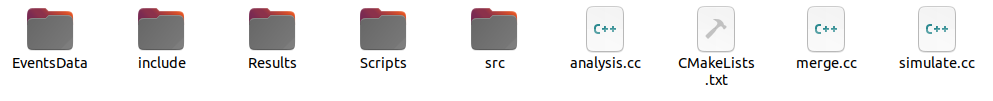
\includegraphics[width=13cm, height=1.3cm]{SourceDir.png} % we give jus a name because we set the path of images with \graphicspath{{images/}}
    \centering
	\caption{DoseCalcs code main directory } 	% caption at the botom if we need it in the top we have to use it befor \includegraphics	
	\label{SrcDir}

\end{figure}
\begin{figure}[H] % its need \usepackage{float} package
	%JPG is Best choice if we want to insert photos. PNG is Best choice if we want to insert diagrams (if a vector version could not be generated) and screenshots
	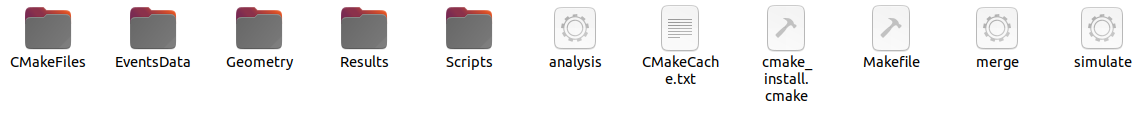
\includegraphics[width=14cm, height=1.5cm]{BuildDir.png} % we give jus a name because we set the path of images with \graphicspath{{images/}}
    \centering
	\caption{DoseCalcs code \textit{build} directory } 	% caption at the botom if we need it in the top we have to use it befor \includegraphics	
	\label{BuildDir}

\end{figure}
\begin{figure}[H] % its need \usepackage{float} package
	%JPG is Best choice if we want to insert photos. PNG is Best choice if we want to insert diagrams (if a vector version could not be generated) and screenshots
	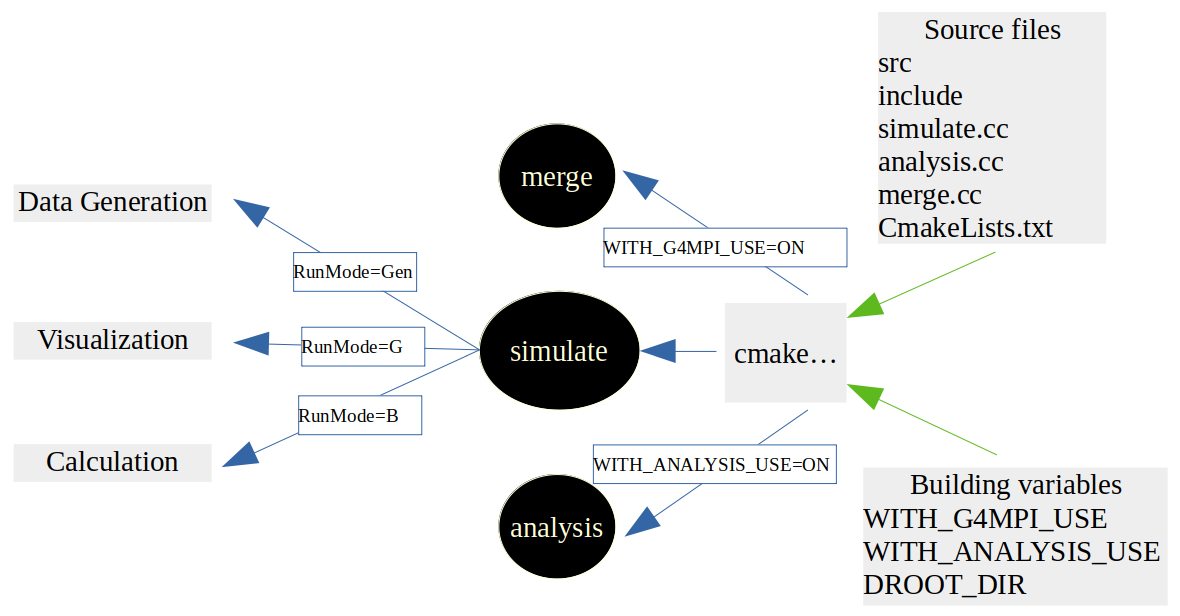
\includegraphics[width=11cm,height=6cm]{DoseCalcsBuilding.png} % we give jus a name because we set the path of images with \graphicspath{{images/}}
    \centering
	\caption{Schematic of DoseCalcs building and running tasks using cmake program. DoseCalcs can be run for three run modes, Gen for data generation, G for geometry graphical visualization and B for calculation. This is for sequential and multi-threading computation modes, however, the G run mode can't be used in MPI computation mode.}
	\label{BuildExecDoseCalcs}
\end{figure}

The build step is performed by setting the variables shown in figure \ref{BuildExecDoseCalcs} to ON or OFF according to the simulation needs. The use of ROOT and MPI requires the installation path of these libraries to be given with -DROOT\_DIR and -DMPI\_DIR variables while building the code. To achieve the simulation task, there are two files that can be considered as principal code inputs, macro command file and geometry file as shown in the figure \ref{BuildExecDoseCalcs}.

The DoseCalcs execution scenario can be done in three computation modes : sequential (SEQ), multi-threading (MT) and Message Passing Interface (MPI). For each scenario three run modes are available, for data generation mode (Gen), calculation mode (B), and graphical visualization mode (G) only for (SEQ) and (MT) scenarios. After commands parameters initialization by messenger classes, the simulation needs five data types which are used in the five simulation steps, material and geometry constructing, physics setting, source defining, simulation run and scoring, and results analysis. Each simulation step is performed basing on the appropriate commands. In figure \ref{DoseCalcsOrganigram}, we describe in details these steps. 

\begin{figure}[H] 
	\includegraphics[width=15cm,height=20cm]{DoseCalcsOrganigram.pdf} 
    \centering
	\caption{DoseCalcs code organigram based on Geant4, showing all the implemented steps that DoseCalcs passes through to simulate a problem and produce desired results.}
	\label{DoseCalcsOrganigram}
\end{figure}

\subsection{Initialization}

DoseCalcs code reads the input commands defined in the macro file by the following messenger classes, \textit{G4TMessenger}, \textit{G4TPhysicsMessenger}, \textit{G4TSourceMessenger} and \textit{G4TGeometryMessenger}.
The macro file is an ASCII file based on the Geant4 macro syntax. The code loads this file to initialize the simulation by selecting the parameters from commands given in this file, then avoiding the need to recompile the source code for any change in the simulation.
The messenger classes read macro commands defined in the macro file as shown in figure \ref{DoseCalcsOrganigram}. These objects send each command value to the appropriate class that are \textit{G4TVolumeConstruction}, \textit{G4TPrimaryGeneratorAction}, \textit{G4TUserPhysics}, \textit{G4TRunAction}, and \textit{G4TRootAnalysis}.

\subsection{Construct materials}

The materials are built using a set of \textit{/MaterialData/} macro commands. DoseCalcs materials can be created either by adding elements and materials each with corresponding data then setting the mass fraction per cent (in the compound) or atoms number (in the molecule) for each one. This is performed by using the following commands \textit{/MaterialData/createElement}, \textit{/MaterialData/createMaterial} and \textit{/AddComponents}. A second way consists of using the NIST \cite{NISTDataBase} material database by setting the NIST material name with the command \textit{/MaterialData/setNistMaterialName}.

In Fact, the material building is essential to construct world volume in STL solid type. Except TEXT and GDML geometry types that use all geometry and material data including world, from TEXT or GDML file.

\subsection{Construct geometry}

In terms of geometry construction, DoseCalcs final Volume is constructed by building in this order, world volume, solids, and volumes. Materials should be created before. DoseCalcs groups these steps in \textit{/GeometryData/} commands, where for world building user should use the command \textit{/GeometryData/createWorld}. Solids are built by use of \textit{/GeometryData/createSolid} command, and volumes construction is achieved by calling the following command \textit{/GeometryData/createVolume}.

Generally, the geometry construction is done by \textit{G4TVolumeConstruction} class, which contains the principal methods: \textit{Construct()}, \textit{ConstructTextGdmlGeometry()}, \textit{ReadSTLGeometry()}, \textit{ConstructGeometryFromCommands()}, \textit{ConstructSDandField()}, \textit{GetRegionAbsolutePosition()}, \textit{ConstructWorldPhysicalVolume()}, and points to several classes to perform multi geometry formats reading and constructing. These classes construct geometry by use of C++ internal implementations or by reading a specific files if required. GDML, TEXT and STL geometry files format can be constructed by our DoseCalcs code. Besides the command file, GDML, TEXT and STL geometry is constructed by reading a specific file that contains the needed shapes and materials data implemented in appropriate format.

DoseCalcs code provides 4 geometry formats handled by several developed classes and methods. Where the geometry building tasks are launched by setting two principal commands \textit{/GeometryData/createSolid} and \textit{/GeometryData/createVolume}. In fact, DoseCalcs can build solids either by C++ coding lines or by reading an STL file. And this is invoked by user just with setting \textit{/GeometryData/createSolid} which needs to specify the solid type, i.e. STL, Box, Tube, Sphere, Para, Trd, Orb, and Ellipsoid. In Addition, user needs two solids to create the third which can be union, or intersection or subtraction of the two solids. The command must be followed by name and shape parameters. For STL type it must be followed just by the solid name and file path of STL file. As a result, this allows to implement the STL geometry as an input geometry file by calling the interface class named \textit{G4TStlToGdml} which handles this format.

Also, the volume can be created using \textit{/GeometryData/createVolume} command. For the solid types cited above, the parameters should be the volume data such as, volume name, material name, mother volume name, position and rotation inside the mother volume, followed by the distance and the angle units. As a consequence, with this command, the STL solid data are read by \textit{GetSolidFacetData()}, and besides the constructed materials, the STL file is converted to GDML file format named by volume name which is passed to \textit{/GeometryData/createVolume} by \textit{StlToGdml()}. Based on mother volume name, position and rotation, the new resulted volume read from the new GDML file by means of \textit{getLogicalVolFromGDMLFile()} is added to the world volume which represents the entire geometry. 

In consequence, the mentioned solid types require firstly, the World volume construction. This can be done by \textit{/GeometryData/createWorld} command, which invokes the \textit{ConstructWorldPhysicalVolume()} method. This command takes as parameters volume name, material name, box half size in X, Y and Z and distance unit. Of course, the material with the passed name should be created before by \textit{/MaterialData/} commands.

By setting GDML or TEXT type as a first parameter of \textit{/CreateVolume} the \textit{ConstructGDMLTEXTVolume()} method is called, where the construction of volumes is done by \textit{G4TGDMLTEXTVolumeConstruction}, using \textit{G4tgbVolumeMgr} and \textit{G4GDMLParser} Geant4 classes for TEXT and GDML manipulation respectively. The principal method in this class is \textit{ReadGeometryFile()}. This method reads GDML or TEXT file given by the second command parameter, which extracts and saves all the volume's data. Each created volume will be assigned to the sensitive detector by the method \textit{ConstructSDandField()}.

The GDML format description of a volume consists of the description of : shape, rotation, position, and material data. All these properties are implemented in the GDML format and one file must contain all volumes as well as the world volume, which means that DoseCalcs takes the entire geometry from this file, without need to construct world volume by \textit{/GeometryData/createWorld}. The same procedure is done with TEXT files.

\subsection{Construct source}

Monte Carlo simulation needs to specify events initial data, in DoseCalcs, this data are generated in a separate execution as shown in figures \ref{BuildExecDoseCalcs} and \ref{DoseCalcsOrganigram}. DoseCalcs uses initial data generated Directly in the beginning of events simulation, and indirectly by using initial data generated in data files. Separating initial data generation and simulation is found useful in regard to the CPU time-consuming either in generation or simulation of huge number of events. Additionally, one can generate all needed data in one execution, to be used in multiple simulations. However, the direct and indirect generation run mode is available for running in multi-threading and MPI computation modes. 

Generation of events initial data is done with the help of \textit{EventsDataGeneration} class, which is instantiated after geometry construction by calling \textit{GenerateEventsData()} method. This method is considered as an interface to the \textit{EventsDataGeneration} class, which contains \textit{GeneratePositionData()} to generate events initial positions inside the source region volume by Monte Carlo method, \textit{GenerateEnergyData()} to generate events initial energies, and \textit{GenerateMomentumDirectionData()} for momentum directions generating according to the distributions names. The data are defined in input macros file. As shown in figure \ref{BuildExecDoseCalcs}, the source events data generation is activated only if the chosen [Run Mode] is "Gen".

The five principal \textit{/SourceData/} commands that hold source parameters, such as events particle names, initial positions, initial energies, initial momentum directions and number of data to generate are \textit{/SourceData/setEventsParticleNameData}, \textit{/SourceData/setEventsInitialPosData}, \textit{/SourceData/setEventsInitialEneData}, \textit{/SourceData/setEventsInitialMomDirData} and \textit{/SourceData/useDataGenerationFiles} respectively.

Positions Generation : The method \textit{GeneratePositionData()} is used to generate the positions coordinates in the source volumes and the corresponding parameters passed in DoseCalcs input file, such as region name, box half dimensions hx, hy and hz. The command takes the first parameter length unit, then "Volume" word, which indicates that the volumes where we want to generate data is a volume with non-uniform shapes, followed by source volume name and the corresponding hx, hy and hz. Additionally, to generate initial positions in more than one volume name, the command support more than one source volume data by adding the second source volume name followed by the corresponding hx, hy and hz, and so on... This makes initial positions generation in multiple sources easy and simple with one command.   

The generation of initial positions in volumes with non-uniform shapes is done with Monte Carlo Rejection method \cite{ExplorMonteCarlo}, where volume shapes are created by GDML, TEXT and STL files.

\begin{figure}[H] % its need \usepackage{float} package
	%JPG is Best choice if we want to insert photos. PNG is Best choice if we want to insert diagrams (if a vector version could not be generated) and screenshots
	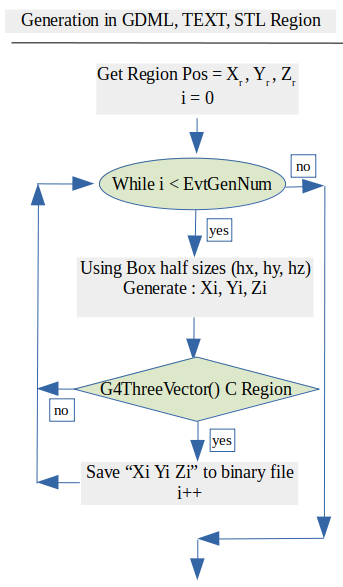
\includegraphics[width=7cm,height=10cm]{DataGenOrganigram.png} % we give jus a name because we set the path of images with \graphicspath{{images/}}
    \centering
	\caption{Flowchart of sampling algorithm used to generate initial position in a source region volume.} 	
	\label{DataGenAlgoOrganigram}

\end{figure}

The initial positions generation is passed through the steps described in figure \ref{DataGenAlgoOrganigram}. The source region absolute position is given by \textit{GetRegionAbsolutePosition()} method from the \textit{EventsDataGeneration} class which returns the \textit{G4ThreeVector(Xr, Yr, Zr)}. Lets consider that the source region is located in the world volume by GeneratePositionData() method, and surrounded by a box with half sizes (hx, hy, hz) passed with \textit{/SourceData/setEventsInitialPosData}. Immediately, an infinity loop is opened, in each turn, a position vector coordinates Xi, Yi, Zi are generated randomly using Monte Carlo rejection method \cite{ExplorMonteCarlo} with the following sampling equations:

\lstset{style=MyCodeStyle}

%\begin{lstlisting}[caption=Initial position coordinates generation]
\begin{lstlisting}
Xi = (Xr - hx) + G4UniformRand()*(2*hx);
Yi = (Yr - hy) + G4UniformRand()*(2*hy);
Zi = (Zr - hz) + G4UniformRand()*(2*hz);
\end{lstlisting}

Then we test if the generated position belongs to the source volume by using the Geant4 class \textit{G4Navigator}:

%\begin{lstlisting}[caption=Position volume localization code]
\begin{lstlisting}
G4Navigator* aNavigator = new G4Navigator();
Region = aNavigator->LocateGlobalPointAndSetup(G4ThreeVector(Xi,Yi,Zi))->GetLogicalVolume()->GetName();
\end{lstlisting}

If the \textit{G4ThreeVector(Xi, Yi, Zi)} is inside the shape of the region source, the Region will be pointing to the source region name, then it will be saved as a line of "X Y Z" to a binary file (ie. \textit{Pos\_Liver\_Volume\_3000000.bin}). If the point generated is out of the region source shape, the generation of new position takes place and so on until saving the needed number of positions to the file. This means that these instructions are re-executed until the number of initial positions saved in .bin file reaches the number given by the first parameter of \textit{/SourceData/useDataGenerationFiles} command. 

For events initial energy generation, the method \textit{GenerateEventsEnergy()} from \textit{EventsDataGeneration} class is used to generate values according to the chosen distribution name and corresponding parameters of \textit{/SourceData/setEventsInitialEneData} command, which requires the energy unit as first argument , followed by distribution name. The available distribution names are Mono, Uniform, Gauss and Rayleigh. When the name of a distribution is passed, it must be followed by its corresponding parameters.
 
For events initial momentum direction generation, the method \textit{GenerateEventsMomDir()} is called to sample the momentum direction components according to the chosen distribution name and corresponding parameters of \textit{/SourceData/setEventsInitialMomDirData} command. This command takes as a first argument the angle unit, followed by distribution name. DoseCalcs code provides the following distribution names, Isotropic, Uniform, and Directed. As for energy generation the command requires the distribution parameters to be passed just after the chosen name.

The data files nomenclature used by DoseCalcs is based on four principal inputs such as data type, distribution name, a value related to this distribution and events number to generate. As a consequence, the file name is constructed in the same manner either for creation during data generation or for reading during simulation process. This nomenclature is used to know clearly which data file to use for the simulation, as well as avoiding the regeneration of the same data with the same name.

After setting the needed source commands, the generation of positions, energies and momentum directions is activated by setting both the second, third and fourth parameters of \textit{/SourceData/useDataGenerationFiles} command to "yes" to invoke \textit{GeneratePositionData()}, \textit{GenerateEnergyData()} and \textit{GenerateMomentumDirectionData()} methods respectively. Note that all the discussed indirect generation tasks using data files are performed by setting the command \textit{/SourceData/useDataGenerationFiles}. Where the direct events data simulation can be done just by unsetting the \textit{/SourceData/useDataGenerationFiles}, then no events data are generated and saved to be used after.

\begin{figure}[H] \centering
    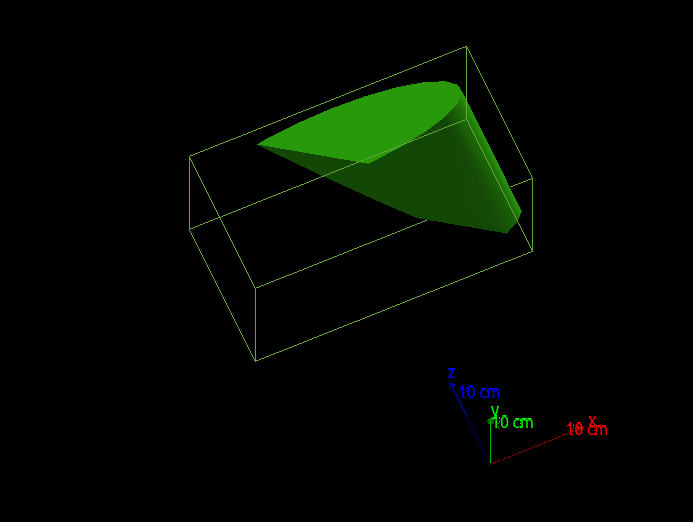
\includegraphics[width=8cm,height=7cm]{BoxSurrendVolume.png}
    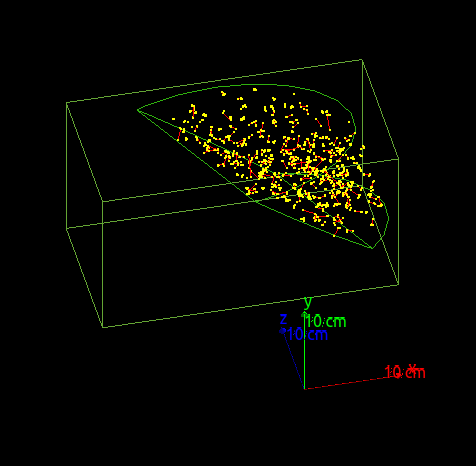
\includegraphics[width=8cm,height=7cm]{BoxPointsTestVisualization.png} 
    \caption{Visualization of surrounded source volume by box before initial positions generation (left), and recorded initial positions after generation step (right).}
    \label{VisVolumeAndTestPoint}
\end{figure}

In the case of the initial positions generation, the box dimensions must be such as the box surrounds the source region as exactly as possible, in order to reduce the generation CPU time. Therefore, the user can use \textit{/SourceData/showSourceBox} command to visualize the enclosing box in the entire geometry as shown in figure \ref{VisVolumeAndTestPoint} (left image), then fine tuning of the box dimensions must be done before generation tasks. The last command invokes \textit{ShowBoxVolume()} method to draw the box volume. Moreover, if the user wants to visualize the initial positions, by setting the command \textit{/SourceData/testEventsInitialPositions} and launching the simulation process, the result will be as shown in figure \ref{VisVolumeAndTestPoint} (right image). This command deactivates the transport process in all the body and only the starting source points are shown. Finally, these two commands are useful to verify that the initial positions are well generated in the desired Region volume. 

\subsection{Construct Physics}

Geant4 toolkit provides various physics processes for different particles, each process can be registered with various models \cite{PhysicsRefGuide}.
All DoseCalcs physics is implemented in \textit{G4TPhysics} class, which contains three principal methods, \textit{ConstructParticle()} which constructs all the particles that will be simulated, \textit{ConstructProcess()} dedicated to build the physics related to the constructed particles, and \textit{SetCuts()} to stop secondary production.

Below a threshold energy given by setting a cut in range or in kinetic energy, the secondary particles are simulated as continuous energy loss by the incident particle, this has no significant effect on the simulation results. Above this threshold, the secondary particles are explicitly generated and followed.

By reading the physics commands arguments sent by \textit{G4TPhysicsMessenger} class to the \textit{G4TPhysics} object, the code uses the selected set of physics constructors to be used in simulation. This can be done by setting the \textit{/PhysicsData/setPhysics} command parameter to one of electromagnetism physics constructors provided by Geant4 physics list (i.e. : EMS, EMO2, EMO1, EMO3, EMO4, Livermore, Penelope).

The performance of any Monte Carlo simulation will be poor if all the secondary particles are simulated and tracked. In order to reduce the simulation time, we use cut in range (distance cut ) or energy threshold (energy cut). The cuts are defined for electrons, positrons, gamma and protons. To determine the cuts values for the simulated particles, the command \textit{/PhysicsData/setCutsData} must be set, the code uses by default the distance cut value that it's converted to a cut in energy internally by Geant4 and vice-versa\cite{PhysicsRefGuide}. If the distance cut is not passed, the energy cut value is set to the default minimal energy. If both cuts are not passed, the default range cut value for electrons and photons is 1 mm, and according to material specification, it is converted to the energy threshold. In Geant4, the energy threshold can be 1 keV or larger \cite{PhysicsRefGuide}.

A useful command used to generate macroscopic cross-sections tables in text format, is \textit{/PhysicsData/GenerateCrossSectionFor}, which takes as arguments the particle name,and energy unit followed by a list of energies where the cross-section will be computed. Then, for each created material in the geometry, a table of macroscopic cross-sections will be created. It contains columns of all processes to be simulated for particle name and for all set energies, and written to the \textit{CrossSectionData} file.

In the current version of DoseCalcs code, the variance reduction techniques are not applied to the simulated problems.

\subsection{Run and Score} 

When the geometry and physics has been constructed, the simulation process begins by creation of an object from \textit{G4TRunAction} class. In this class, the \textit{BeginOfRunAction()} method contains initialization values of all data needed to perform a simulation. DoseCalcs uses one run object in sequential computation mode which means one thread, the same for MPI computation mode, each rank simulates one run sequentially and the total number of runs will be the number of ranks, each rank simulates a specific source data separately. Likewise in multi-threading computation mode,  simulation events total number is divided on the number of threads, and each thread simulates corresponding events number with the same source data.

At the beginning of a simulation process, after run initialization, each thread reads the data files and fills the position, energy and momentum arrays of size equal to the events number entrusted to this thread. Then it reads the appropriate lines from the data files, in order to avoid the recurrence of an event's simulation with the same initial data. In consequence, it is recommended that the total number of simulated events by all threads must be equal or less than the number of lines in the data files. Note that each line in a data file corresponds to an event position, energy or momentum direction.

In DoseCalcs, an event is represented by an object of \textit{G4TEventAction}, which is initialized by \textit{BeginOfEventAction()} method. At each interaction step of this event or one of its secondaries, the \textit{ProcessHits()} method is invoked from the \textit{G4TSD} object, which sets a \textit{G4THit} object that contains the deposited energy and the interaction volume name.
In fact, the energy deposited in a volume name is considered as a main variable in internal dosimetry Monte Carlo simulation, which is needed to be scored at each step in \textit{ProcessHits()} method. Geant4 provides \textit{GetTotalEnergyDeposit()} method defined in \textit{G4Step} class, which returns the energy deposited during an interaction step. Note that the \textit{G4THit} data are accumulated for each step of an event, as well for each event in a run.

At the end of a run, for worker thread, the \textit{CreateThreadRegionResultFile()} is called to write thread calculated data as lines of all defined regions data, each line contains region name, total energy deposited in, the square of total energy deposited and total number of steps simulated in this region.
For the master thread, the \textit{CreateSimulationDataFile()} is called to generate a file called \textit{SimData} containing simulation data with the needed parameters to generate the final results file by means of \textit{G4TResultCalculation} object, and to be used also by \textit{G4TRootAnalysis} as an input file to generate graphs, histograms and tables.

In \textit{G4TResultCalculation} class, three reading methods are to be called first, \textit{ReadSimulationData()}, \textit{ReadTissueAndRadiationFactorsFiles()} used in calculating equivalent and effective dose, and \textit{ReadThreadRegionResult()}, with the objective of getting all the needed data, then merging the threads results and calculating the final simulation results by the \textit{QuantitiesCalculation()} method.

The calculation of internal dosimetry quantities such as AD, AF, SAF, S, H and E in each region is based on the energy deposited in each region for each thread file. Also the statistical data in each region, are calculated based on the square of deposited energy and number of steps in each region. These calculation tasks are done in the \textit{QuantitiesCalculation()} method in \textit{G4TResultCalculation} object for each region (r) using the following equations :

\begin{equation}
    \label{eq:AD}
    AD_r = \frac{ED_{r,t}}{M} , \quad in \quad Gray 
\end{equation} 
\begin{equation}
    \label{eq:AF}
    AF_r = \frac{ED_{r,t}}{TEE_s} 
\end{equation} 
\begin{equation}
    \label{eq:SAF}
    SAF_r = \frac{AF_r}{M_r}  , \quad in \quad kg^{-1} 
\end{equation} 
\begin{equation}
    \label{eq:S}
    S_r = \frac{AD_r}{N}  , \quad in \quad Gray/event 
\end{equation} 
\begin{equation}
    \label{eq:H}
    H_r = AD_r\times Wr  , \quad in \quad Sv 
\end{equation} 
\begin{equation}
    \label{eq:E}
    E = \sum H\times Wt  , \quad in \quad Sv
\end{equation} 

Where,\\
$ \text{M}_{r} $ : Region Mass (in kg) \\
$ \text{ED}_{r,t} $ : Total energy deposited in region r (in MeV) \\
$ \text{TEE}_{s} $ : Total Emitted Energy from source s (in MeV)  \\
N : Number of Events \\
Wr : Radiation Factor \\
Wt : Tissue Factor \\

For accuracy calculation : 

\begin{equation}
    \label{eq:Mean}
    \text{Mean} = \overline{ED_{r}} = \frac{1}{N_{I,r}} \sum_{i=1}^{N_{I,r}} ED_{r,i}.
\end{equation} 
\begin{equation}
    \label{eq:Var}
    \text{Variance} = s_r^2 = \frac{1}{N_{I,r} - 1} \sum_{i=1}^{N_{I,r}} \left ( ED_{r,i} - \overline{ED_{r}} \right )^2 =\frac{1}{N_{I,r} - 1} \left ( \sum_{i=1}^{N_{I,r}} ED_{r,i}^2 - N_{I,r}\overline{ED_{r}}^2 \right ).
\end{equation} 
\begin{equation}
    \label{eq:SD}
    \text{Standard deviation} = \sqrt{s_r^2} 
\end{equation} 
\begin{equation}
    \label{eq:RelSD}
    \text{Relative standard deviation (\%)} = \frac{\sqrt{s_r^2}}{\overline{ED_{r,t}}}\times 100
\end{equation} 

%Standard deviation =
%Relative error = Standard deviation / Mean

Where $N_{I,r}$ is the Number of Interactions sampled in the region r and the $ED_r$ is the average energy deposited in this region.

\definecolor{ColorTextFile}{rgb}{0.94, 1.0, 1.0}

\begin{figure}[H] 
\begin{adjustbox}{max width=\linewidth, margin= 5 , bgcolor = ColorTextFile ,  margin= 1, bgcolor = black}
  \RecustomVerbatimCommand{\BVerbatimInput}{BVerbatimInput}%
  {fontsize=\footnotesize,
  frame=lines,
  framesep=2em,
  rulecolor=\color{Gray},
  label=\fbox{\color{Black}ResultsData},
  labelposition=topline,
  }
  \BVerbatimInput{./ResultsData}
\end{adjustbox}
  \caption{Results file for one simulation with two scored quantities, SAF and S, in four Volumes. The simulation starts with 1 MeV Mono energetic gamma, with isotropic momentum direction, and distributed in Liver. 40000 events were simulated, where the multi-threading (MT) mode is used, the simulation execution requires about 0.05 minutes. Additional information can be found in the header line.} 
  \label{ResultFile}
\end{figure}

Finally, the results file as shown in figure \ref{ResultFile}, is generated by the \textit{GenerateRegionResultFile()} method in \textit{G4TResultCalculation} class. The printed quantities are those passed by command \textit{/RunAndScoreData/setQuantitiesToScore}, in volumes given by \textit{/RunAndScoreData/setVolumesToScore}. Where for each simulation, i.e source volume, particle and energy combination, the obtained scores are appended to results file. The generated data are written in a simple format, first line as a simulation header file which contains simulation data such as scored quantity, source volume name, particle name, etc. followed by data lines, each line contains the results for a scored volume. 

\subsection{Generate Data Tables and ROOT graphs and histograms} 

The purpose of a graph or histogram is to present data that are too numerous or complicated to be described adequately in the text and in less space. In order to make graphs and histograms easily, \textit{G4DoseCalcsAnalysis} class has been developed as a direct interface to ROOT Analysis System \cite{ROOT}. This class serves to generate graphs according to the \textit{/AnalysisData/generateSelfCrossGraphs} command parameters. Note that this command parameters such as graph type, comparing type, reference name, reference file path, and other analysis commands parameters, must be given in the macros file DoseCalcs save them to the simulation data file \textit{SimData} created by \textit{CreateSimulationDataFile()} method at the end of simulation run. This file is to be reused beside the results file like the one shown in figure \ref{ResultFile} created by \textit{CreateThreadRegionResultFile()} as an input file for analysis tasks. However, the parameters in \textit{SimData} file should be adjusted to create the desired analysis tasks by \textit{G4DoseCalcsAnalysis}. 

First, the graphs are created under two principal conditions:

-The user must build the DoseCalcs code with option WITH\_ANALYSIS\_USE=ON and set the ROOT\_Dir=/../../root as shown in figure \ref{BuildExecDoseCalcs}. This will build an executable called analysis, the execution of analysis generates graphs and histograms.

-The first \textit{/AnalysisData/generateSelfCrossGraphs} parameter should point to Result or Result\_Reference value, and if the value is Result\_Reference, the reference data file should be given and written in a specific text format in order to be readable by \textit{G4DoseCalcsAnalysis} class.

The graphs that can be generated are for self-absorption and cross-irradiation either for results and reference or just for results by invoking the \textit{GenerateSelfCrossGraphs()}. Also, and by \textit{/AnalysisData/generateRelativeErrGraph} command, the relative error graph can be generated by using the results and reference data and invoking \textit{GenerateRelErrGraph()}.

With \textit{/AnalysisData/generateRelativeSDevGraph}, another type of graphs is the relative standard deviation percent as a function of energy, which is given for each source region, in order to show how this parameter changes with energy and target regions variability.

In the context of data analysis for internal dosimetry purpose, the user can generate a graph of a quantity i.e. SAF, in function of either volume, mass, density, and distance between the source and target, by using /AnalysisData/generateVariableRegionGraph command, which takes the variable name (i.e. Mass, Volume, Density and Distance) as an argument. This will show clearly how a dosimetry quantity value changes between targets and sources, and give insight about the parameter that affects this scored quantity.

The generated positions, energies and momentum directions data can be viewed in histograms using the following \textit{/AnalysisData/generateEventsDataHisto} command, which invokes :\\
\textit{GenerateEnergiesHist()} to use the data created in energies file,\\
\textit{GenerateMomentumDistributionsHist()} to use the data created in momentum directions file, and \\
\textit{GeneratePositionsHist()} to use the data created in positions file.\\
To invoke these methods, one should look out the event's data files paths defined in simulation data file. Likewise, to well generate data histograms, the number of events data in these files must be the same. 

As well, the generated \textit{CrossSectionData} file can be read to generate macroscopic cross-sections graph by \textit{GenerateCrossSectionGraph} method for each particle and material. In addition, the phantom region's data (Region names, mass, volume and density), macroscopic cross sections, DoseCalcs results and reference data are generated in Latex tables formats by \textit{GenerateLatexFormatTables()}, in order to facilitate the use of application results.

Note that, the graphs parameters can be set or activated by the command \textit{/AnalysisData/setGraphsParameters}, which takes as arguments, "yes" or "no" flags to activate logarithmic scale for x-axis and y-axis, to show x-y grid, to show title, and graph legend position which can be either, RightTop, RightBottom, LeftTop, RightBottom, MiddleTop or MiddleBottom. The last argument is for graphs and histograms files extension, which can be either, .pdf, .ps, .jpeg or .root .

\section{ Execution } 

Of course, DoseCalcs code building requires Geant4 to be installed first, and it is preferred that Geant4 be built for multi-threading computation mode. Then, to run DoseCalcs sequentially, the number of threads to be passed to \textit{/RunAndScoreData/setThreadsNumber} should be set to 1.

With a command line processing interface, the execution is done in multi-threading or sequential computation mode by typing the following command :
\begin{lstlisting}
./simulate [Run Mode] [macros file] [events number]
\end{lstlisting}

In MPI computation mode, the mpiexec or mpirun execution command should be set firstly as given in the following command :
\begin{lstlisting}
/path/to/mpirun -np [number of ranks] ./simulate [Run Mode] [macros file] [EventsNumber]
\end{lstlisting}

The [Run Mode] can be one of B(batch), G(Graphical) or Gen(Generation) modes. The Graphical mode is used to visualize(v) the geometry read by DoseCalcs, as well as to test the events initial positions by setting the command \textit{/TestEventsInitialPositions}. It allows also the box dimensions visualization by setting the command \textit{/ShowSourceBox} in the macro file. As mentioned before, the graphical mode can be used only in sequential and multi-threading computation modes. However, MPI computation mode is directed just for Batch and Generation Run Modes. The Batch run mode is dedicated to simulation and scoring and the Gen run mode is used for events data generation such as initial positions, energies and momentum directions. 

\begin{figure}[H] 
    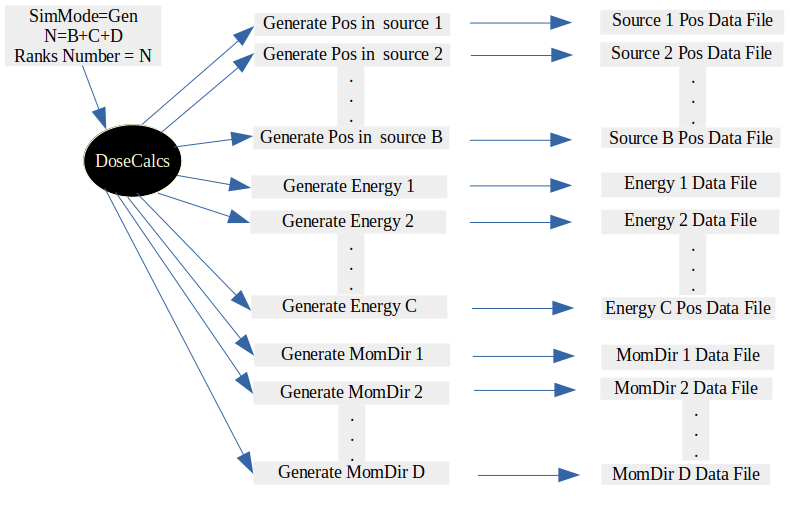
\includegraphics[width=12cm,height=7cm]{SimModeGen.png}
    \centering
	\caption{Chart of DoseCalcs running for data generation tasks, the same number of the generated data on each rank is given in DoseCalcs input file. } 
	\label{SimModeGen}
\end{figure}

\begin{figure}[H]
    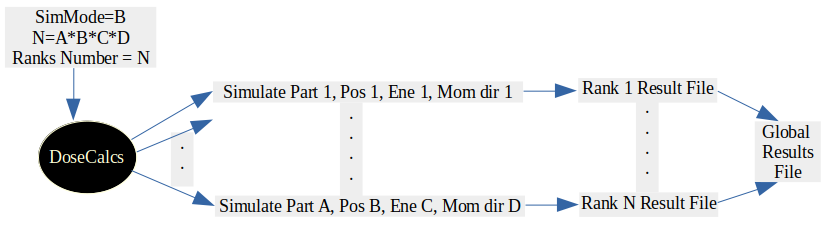
\includegraphics[width=12cm,height=3.6cm]{SimModeB.png}
    \centering
	\caption{Chart of DoseCalcs running for simulation tasks, the same number [EventsNumber] of events is simulated on each rank.}
	\label{SimModeB}
\end{figure}

In MPI computation mode, the simulation and data generation events are distributed on all the ranks. Supposing that we have as an input, A particles(Part), B source Regions(Src), C energies(Ene) and D momentum directions(MomDir), the data generation tasks are distributed among the ranks as shown on figure \ref{SimModeGen}. As a consequence, the number of ranks needed to generate these events data is $N=B+C+D$, where each rank generates a specific data file, whereas the number of ranks needed for simulations will be the number of combinations Part-Src-Ene-MomDir which is $N=A\times B\times C\times D$ as shown in figure \ref{SimModeB}. Therefore, it's recommended to specify the right number of ranks according to inputs given in the macros file and also to the run mode (B or Gen) before launching DoseCalcs. To perform these N simulations on ranks, the command \textit{/RunAndScoreData/setSimNumOnRanks} must be set to "m", which means multi-simulations on ranks. An Additional option, is the capability to simulate one Part-Src-Ene-MomDir combination ($A=B=C=D=1 \Rightarrow N=1$) on all ranks by setting \textit{/RunAndScoreData/setSimNumOnRanks} to "o", which means one simulation on ranks, where the simulated events data are not repeated, each rank reads a specific data lines in initial positions, energies and momentum directions data files. Note that the total number of simulated events in this case for one simulation (for one combination) is $\text{TotalEventsNumber}=N\times\text{[EventsNumber]}$, instead of "m" option, the number of simulated events for each combination is [EventsNumber].

In multi-threading or sequential computation mode, just the first combination Part-Src-Ene-MomDir of source data will be simulated in Batch run mode, whereas the Generation run mode serves to generate all source data sequentially. In multi-threading computation mode, the EventsNumber passed in execution command is simulated for each thread, the same for MPI which is considered to be simulated in each rank. The total number of simulated events is the EventsNumber multiplied by thread number or rank number for multi-threading and MPI computation modes respectively. Note that this total number should not exceed the maximum G4int value.

In the case a simulation on a rank crashed due to memory problem, the \textit{merge} executable which is built as a helper for results calculation in MPI computation mode, can be used to generate global results from ranks that achieved successfully the simulation and have produced the results file related to their own rank.

\section{ Results and discussion } 

Mathematical geometries of the phantom regions are used. They are based on the data published in \cite{MIRDRefSAFData}, \cite{G4HumanPhantom} in GDML format file. On table \ref{MIRDMatComp} we present the MIRD phantom materials composition. The phantom regions name and the corresponding data such as mass, volume and density used in the simulation geometry, are given in table \ref{RegionImpleData}. In order to respect the reference simulation source data, the simulated particle was gamma with Mono type energies in MeV : 0.01, 0.015, 0.02, 0.03, 0.05, 0.1, 0.2, 0.5, 1. The momentum direction distribution was isotropic. 

The physics used to simulate the electromagnetic interactions were EMO3 (\textit{electromagneticoption$\_$3} constructor). For Photons, the (e-,e+) pair production is implemented by the \textit{BetheHeitler} model, Compton scattering is implemented by the \textit{Klein-Nishina} model, and Photo-electric effect and Rayleigh  scattering are both handled by the \textit{Livermore} models. For electrons and positrons, multiple Coulomb scattering process is handled by the \textit{Urban} model, Bremsstrahlung is implemented by the \textit{eBremSB} and \textit{eBremLPM} models, ionization is modeled by the \textit{Moller-Bhabha formulation}, and positron annihilation is implemented by the \textit{eplus2gg} model.

\begin{table}[H]
\centering
\caption{MIRD Phantom material composition, data correspond to weight fractions in percent.} 
\begin{tabular}{llll}
\hline
\textbf{Element} & \textbf{Skeletal Tissue} & \textbf{Lung Tissue} & \textbf{Total Body} \\ \hline
H                & 7.04                     & 10.21                & 10.47               \\ \hline
C                & 22.79                    & 10.01                & 23.02               \\ \hline
N                & 3.87                     & 2.8                  & 2.34                \\ \hline
O                & 48.56                    & 75.96                & 63.21               \\ \hline
Na               & 0.32                     & 0.19                 & 0.13                \\ \hline
Mg               & 0.11                     & 7.40E-03             & 0;015               \\ \hline
P                & 6.94                     & 0.081                & 0.24                \\ \hline
S                & 0.17                     & 0.23                 & 0.22                \\ \hline
Cl               & 0.14                     & 0.27                 & 0.14                \\ \hline
K                & 0.15                     & 0.2                  & 0.21                \\ \hline
Ca               & 9.91                     & 7.00E-03             & 0                   \\ \hline
Fe               & 8.00E-03                 & 0.037                & 6.30E-03            \\ \hline
Zn               & 4.80E-03                 & 1.10E-03             & 3.20E-03            \\ \hline
Rb               & 0                        & 3.70E-04             & 5.70E-04            \\ \hline
Sr               & 3.20E-03                 & 5.90E-06             & 3.40E-05            \\ \hline
Zr               & 0                        & 0                    & 8.00E-04            \\ \hline
Pb               & 1.10E-03                 & 4.10E-05             & 1.60E-05            \\ \hline
Density          & 1.4862 $g/cm^3$             & 0.2958 $g/cm^3$         & 0.9869 $g/cm^3$        \\ \hline
\end{tabular}
\label{MIRDMatComp}
\end{table}

\begin{table}[H] 
\centering
\caption{Region names implemented in the phantom geometry and the corresponding volume, mass and density.} 
\begin{tabular}{llll} 
\hline 
\textbf{Region Name}         & \textbf{Volume ($cm^3$)}      & \textbf{Mass (kg)}   & \textbf{Density ($g/cm^3$)}                     \\\hline
Adrenal     & 15.7034      & 0.0154977     & 0.9869       \\\hline
Clavicle     & 55.0367      & 0.0817955     & 1.4862       \\\hline
Heart     & 602.992      & 0.595093     & 0.9869       \\\hline
Liver     & 1829.57      & 1.8056     & 0.9869       \\\hline
Lung     & 3387.27      & 1.00196     & 0.2958       \\\hline
Kidney     & 287.955      & 0.284183     & 0.9869       \\\hline
Pelvis     & 218.716      & 0.325056     & 1.4862       \\\hline
Spleen     & 175.728      & 0.173426     & 0.9869       \\\hline
Stomach     & 401.471      & 0.396212     & 0.9869       \\\hline
Thymus     & 25.1327      & 0.0248035     & 0.9869       \\\hline
Pancreas     & 61.0591      & 0.0602592     & 0.9869       \\\hline
Ovary     & 8.34433      & 0.00823502     & 0.9869       \\\hline
SmallIntestine     & 1020      & 1.00664     & 0.9869       \\\hline
UpperLargeIntestine     & 331.281      & 0.326941     & 0.9869       \\\hline
UrinaryBladder     & 248.171      & 0.24492     & 0.9869       \\\hline
MiddleLowerSpine     & 573.68      & 0.852603     & 1.4862       \\\hline
LowerLargeIntestine     & 263.783      & 0.260327     & 0.9869       \\\hline
Uterus     & 71.4062      & 0.0704708     & 0.9869       \\\hline
ArmBone     & 954.58      & 1.4187     & 1.4862       \\\hline
Brain     & 1470.67      & 1.45141     & 0.9869       \\\hline
Thyroid     & 19.3757      & 0.0191219     & 0.9869       \\\hline
Skull     & 638.349      & 0.948715     & 1.4862       \\\hline
UpperSpine     & 133.156      & 0.197897     & 1.4862       \\\hline
LegBone     & 2795.72      & 4.15501     & 1.4862       \\\hline
Head     & 5072.25      & 5.00581     & 0.9869       \\\hline
Trunk     & 43274.6      & 42.0142     & 0.9869       \\\hline
Legs     & 21983.1      & 21.6951     & 0.9869       \\\hline
Skin     & 2790.97      & 2.75441     & 0.9869       \\\hline
Rib     & 696.567      & 1.03524     & 1.4862       \\\hline
Teste     & 37.5326      & 0.0370409     & 0.9869\\ \hline
\end{tabular} 
\label{RegionImpleData}
\end{table}

In order to reproduce results in a good agreement with reference, the dosimetric parameters in the simulated phantom such as mass, should be the same as described in the reference phantom. The organs shape, mass, volume and position are implemented via GDML format. In consequence, they can be slightly different in values compared to the reference data except density, and this can induce small relative differences between the code results and reference ones. In this simulation, we are interested in three organs (Liver, Kidney and Adrenal) as sources and targets during simulation to score the dosimetry quantities. The chosen organs are contained inside the volume of Trunk region which is filled by three materials each with a specific density as shown in table \ref{MIRDMatComp}. The difference between the organs of the same material and density is the volume, then different masses are attributed to different organs which affects the region internal dosimetry quantities. Generally, In the GDML implementation, after fixing the density value we make fine tuning of the volume parameter to give approximately the same mass as given in MIRD phantom \cite{MIRDRefSAFData}.

The history of a photon in the reference data, is terminated while one of the three events occurs, first, if it escapes from the phantom, second, if its energy falls below 4 keV, and third, if its weight falls below $\mathrm{10}^{-5}$. In the latter two cases, the energy is considered to be absorbed locally. Likewise, for the DoseCalcs validation, we set the cut in range and energy threshold for gamma and electron to 0.1 mm and 0.001 keV respectively. This range is too small to the mean free path of photons in these materials. In addition, reference simulation kills the photon if it reaches the phantom boundaries, this can underestimate the absorbed energy because there is no reflection from the world to the phantom. To do so in our simulations, we use the vacuum material (G4\_Galactic of density $g/cm^3$) that fills the world volume, which reproduces the same principle of no interaction and no reflection in and from world volume.

Each rank simulates a couple of Part-Src-Ene-MomDir with 40000000 events, and the total number of the performed simulations was $1\times3\times9\times1 = 27$, one particle, three source organs, nine energies, and one momentum direction. A cluster of 10 nodes with 48 cores was used in our simulations. Note that we rank by core, the maximum number of DoseCalcs simulations allowed on this cluster is 48. 
%Besides this, the Events number should not exceed the max of G4int Geant4 type $(2 147 483 647)$, that's why the number of events in each simulation was fixed to 40000000, which considers the condition $27\times40000000<2 147 483 647$.

\definecolor{ColorTextFile}{rgb}{0.94, 1.0, 1.0}
\begin{figure}[H] 
\centering
\begin{adjustbox}{max width=\linewidth, margin= 5 , bgcolor = ColorTextFile ,  margin= 1, bgcolor = black}
  \RecustomVerbatimCommand{\BVerbatimInput}{BVerbatimInput}%
  {fontsize=\footnotesize,
  frame=lines,
  framesep=2em,
  rulecolor=\color{Gray},
  label=\fbox{\color{Black}macrosGdml.mac},
  labelposition=topline,
  }
  \BVerbatimInput{./macrosGdml.mac}
\end{adjustbox}
  \caption{Validation inputs data defined in macro file of DoseCalcs.} 
  \label{macroFile}
\end{figure}

The DoseCalcs code produces results for most internal dosimetry quantities such as absorbed dose (AD), absorbed fraction (AF), specific absorbed fraction(SAF), S value (S), equivalent dose (H) and effective dose (E). For validation purpose, we choose to calculate the SAF as they are provided by reference study. Since the SAF values depend on photon energy and geometrical parameters, then we just make a tuning of parameters like the organ's volume, shape and internal distance between these organs. So these are the most parameters that can affect agreement between resulted SAF values and the reference data. Moreover, the SAF values are to be distinguished in the two following cases : self-absorption and cross-irradiation. Self-absorption occurs when the target organ is the same as the source one. Whereas the cross-irradiation happens when the target organ is different from the source one. The SAF results values are compared to the reference MIRD SAF data \cite{MIRDRefPhantomData} in order to analyse the differences and fluctuations originated from DoseCalcs code calculations. Physically, the density of the source region material and the particles energy are the most important factors that affect the SAF for both self-absorption and cross-irradiation, because they influence directly the ability of particles to escape from the source organ or penetrate the target organ. On the other hand density of organs and distance between source and the target organs, affect the cross-irradiation SAF.

The DoseCalcs results obtained for self-absorption SAFs and scored for three organs, Liver, Kidney and Adrenal, are presented in table \ref{SelfIrr}. In tables \ref{CrossFromLiver}, \ref{CrossFromKidney} and \ref{CrossFromAdrenal} we summarize the calculated values of SAF for cross-irradiation from source organs Liver, Kidney and Adrenal respectively. These values are compared to the corresponding ones obtained from MIRD reference \cite{MIRDRefPhantomData}. Additionally, the relative error and relative standard deviation percent are given.

\begin{table}[H]
\centering
\caption{Comparison of self-absorption SAF values calculated by DoseCalcs and those of the MIRD reference.}
\begin{adjustbox}{width=\columnwidth,center}
\begin{threeparttable}
\begin{tabular}{lllllllllll} \hline 
\multicolumn{1}{c}{\multirow{2}{*}{\textbf{Region Name}}} & \multirow{2}{*}{\textbf{Method}} & \multicolumn{9}{c}{ SAF Self Absorption with gamma \textbf{Energies in MeV}}       \\ \cline{3-11}
                 \multicolumn{1}{c}{}                             & \multicolumn{1}{c}{}                           & \textbf{0.01}   & \textbf{0.015}   & \textbf{0.02}   & \textbf{0.03}   & \textbf{0.05}   & \textbf{0.1}   & \textbf{0.2}   & \textbf{0.5}   & \textbf{1}       \\\hline 
\multirow{4}{*}{\textbf{Liver}}       & DoseCalcs                                         & 0.536218        & 0.500466        & 0.442905        & 0.30936        & 0.159941        & 0.0948983        & 0.0896701        & 0.089012        & 0.0808983        \\ 
                             & MIRD                                        & 0.536        & 0.496        & 0.434        & 0.297        & 0.152        & 0.0914        & 0.0882        & 0.0885        & 0.0807        \\ 
                             & RD(\%)\tnote{a}                                        & 0.0407463        & 0.900363        & 2.05194        & 4.16172        & 5.22434        & 3.82749        & 1.66672        & 0.578565        & 0.245675        \\ 
                             & Rel SD(\%)\tnote{b}                                          & 0.01        & 0.011        & 0.013        & 0.017        & 0.021        & 0.017        & 0.016        & 0.01        & 0.008               \\\hline 
\multirow{4}{*}{\textbf{Kidney}}       & DoseCalcs                                         & 3.29824        & 2.80777        & 2.13773        & 1.09964        & 0.418557        & 0.238256        & 0.244064        & 0.25383        & 0.22953        \\ 
                             & MIRD                                        & 3.28        & 2.74        & 2.04        & 1.03        & 0.393        & 0.235        & 0.239        & 0.252        & 0.226        \\ 
                             & RD(\%)\tnote{a}                                         & 0.556189        & 2.47321        & 4.79064        & 6.76146        & 6.5031        & 1.3854        & 2.11879        & 0.72631        & 1.5619        \\ 
                             & Rel SD(\%)\tnote{b}                                          & 0.01        & 0.012        & 0.015        & 0.022        & 0.034        & 0.026        & 0.025        & 0.015        & 0.011               \\\hline 
\multirow{4}{*}{\textbf{Adrenal}}       & DoseCalcs                                         & 52.4148        & 34.0331        & 19.9623        & 7.52409        & 2.30845        & 1.3332        & 1.45581        & 1.5463        & 1.33078        \\ 
                             & MIRD                                        & 52.2        & 32.9        & 18.9        & 7.04        & 2.23        & 1.33        & 1.45        & 1.57        & 1.51        \\ 
                             & RD(\%)\tnote{a}                                         & 0.411533        & 3.44404        & 5.62058        & 6.87634        & 3.51776        & 0.240752        & 0.400414        & -1.5093        & -11.869        \\ 
                             & Rel SD(\%)\tnote{b}                                          & 0.011        & 0.015        & 0.021        & 0.037        & 0.062        & 0.046        & 0.045        & 0.028        & 0.021        \\ \hline
\end{tabular} 
\begin{tablenotes}\footnotesize
\item[a] Relative Difference (\%)
\item[b] Relative Standard Deviation (\%)
\end{tablenotes}
\end{threeparttable}
\end{adjustbox}
\label{SelfIrr}
\end{table}


\begin{table}[H] 
\centering
\caption{Cross-irradiation SAF Values from Liver calculated by DoseCalcs and compared to the MIRD reference. } 
\begin{adjustbox}{width=\columnwidth,center}
\begin{threeparttable}
\begin{tabular}{lllllllllll} \hline 
\multicolumn{1}{c}{\multirow{2}{*}{\textbf{Region Name}}} & \multirow{2}{*}{\textbf{Method}} & \multicolumn{9}{c}{ SAF for cross-irradiation from Liver Source with gamma \textbf{Energies in MeV}}       \\ \cline{3-11}
                 \multicolumn{1}{c}{}                             & \multicolumn{1}{c}{}                           & \textbf{0.01}   & \textbf{0.015}   & \textbf{0.02}   & \textbf{0.03}   & \textbf{0.05}   & \textbf{0.1}   & \textbf{0.2}   & \textbf{0.5}   & \textbf{1}       \\\hline 
\multirow{4}{*}{\textbf{Kidney}}       & DoseCalcs                                         & 3.56162e-05        & 0.000932552        & 0.00466864        & 0.0159893        & 0.0208884        & 0.0167583        & 0.0150188        & 0.0141481        & 0.013049        \\ 
                             & MIRD                                        & 0.00083        & 0.00126        & 0.0045        & 0.0157        & 0.0195        & 0.0158        & 0.0136        & 0.0129        & 0.0118        \\ 
                             & RD(\%)\tnote{a}                                         & -95.7089        & -25.9879     & 3.74762        & 1.84287        & 7.12015        & 6.06513        & 10.432        & 9.67488        & 10.5847        \\ 
                             & Rel SD(\%)\tnote{b}                                          & 3.112        & 0.665        & 0.316        & 0.182        & 0.146        & 0.108        & 0.096        & 0.07        & 0.052               \\\hline 
\multirow{4}{*}{\textbf{Adrenal}}       & DoseCalcs                                         & 0.000406109        & 0.00524748        & 0.0144641        & 0.0255523        & 0.0245866        & 0.018958        & 0.0170914        & 0.0164116        & 0.0154254        \\ 
                             & MIRD                                        & 0.00245        & 0.00368        & 0.0136        & 0.0268        & 0.0215        & 0.0161        & 0.0181        & 0.0168        & 0.0156        \\ 
                             & RD(\%)\tnote{a}                                         & -83.4241        & 42.5947        & 6.3536        & -4.65545        & 14.3564        & 17.7517        & -5.57243        & -2.31173        & -1.11949        \\ 
                             & Rel SD(\%)\tnote{b}                                          & 4.011        & 1.207        & 0.773        & 0.621        & 0.579        & 0.43        & 0.389        & 0.281        & 0.198        \\ \hline
\end{tabular} 
\begin{tablenotes}\footnotesize
\item[a] Relative Difference (\%)
\item[b] Relative Standard Deviation (\%)
\end{tablenotes}
\end{threeparttable}
\end{adjustbox}
\label{CrossFromLiver}
\end{table}

\begin{table}[H] 
\centering
\caption{Cross-irradiation SAF Values from Kidney calculated by DoseCalcs and compared to the reference MIRD. } 
\begin{adjustbox}{width=\columnwidth,center}
\begin{threeparttable}
\begin{tabular}{lllllllllll} \hline 
\multicolumn{1}{c}{\multirow{2}{*}{\textbf{Region Name}}} & \multirow{2}{*}{\textbf{Method}} & \multicolumn{9}{c}{ SAF for cross-irradiation from Kidney Source with gamma \textbf{Energies in MeV}}       \\ \cline{3-11}
                 \multicolumn{1}{c}{}                             & \multicolumn{1}{c}{}                           & \textbf{0.01}   & \textbf{0.015}   & \textbf{0.02}   & \textbf{0.03}   & \textbf{0.05}   & \textbf{0.1}   & \textbf{0.2}   & \textbf{0.5}   & \textbf{1}       \\\hline 
\multirow{4}{*}{\textbf{Liver}}       & DoseCalcs                                         & 3.55321e-05        & 0.000933995        & 0.00469021        & 0.016021        & 0.02108        & 0.017003        & 0.0151281        & 0.0142009        & 0.0131008        \\ 
                             & MIRD                                        & 0.00044        & 0.000665        & 0.00468        & 0.0154        & 0.0195        & 0.0153        & 0.0136        & 0.0138        & 0.0122        \\ 
                             & RD(\%)\tnote{a}                                         & -91.9245        & 40.4504        & 0.218077        & 4.03279        & 8.10231        & 11.1307        & 11.2359        & 2.90493        & 7.38336        \\ 
                             & Rel SD(\%)\tnote{b}                                          & 1.247        & 0.263        & 0.125        & 0.072        & 0.058        & 0.043        & 0.038        & 0.028        & 0.021               \\\hline 
\multirow{4}{*}{\textbf{Adrenal}}       & DoseCalcs                                         & 0.00115539        & 0.0251886        & 0.0675812        & 0.0989554        & 0.0692466        & 0.0439754        & 0.0411712        & 0.0406676        & 0.0375683        \\ 
                             & MIRD                                        & 0.0047        & 0.0395        & 0.0811        & 0.0944        & 0.063        & 0.0451        & 0.0348        & 0.0428        & 0.0401        \\ 
                             & RD(\%)\tnote{a}                                         & -75.4173        & -36.2314        & -16.6692        & 4.82565        & 9.9153        & -2.49346        & 18.3082        & -4.9822        & -6.31354        \\ 
                             & Rel SD(\%)\tnote{b}                                          & 2.375        & 0.55        & 0.358        & 0.316        & 0.348        & 0.275        & 0.256        & 0.177        & 0.124        \\ \hline
\end{tabular} 
\begin{tablenotes}\footnotesize
\item[a] Relative Difference (\%)
\item[b] Relative Standard Deviation (\%)
\end{tablenotes}
\end{threeparttable}
\end{adjustbox}
\label{CrossFromKidney}
\end{table}

\begin{table}[H] 
\centering
\caption{Cross-irradiation SAF Values from Adrenal calculated by DoseCalcs and compared to the reference MIRD. } 
\begin{adjustbox}{width=\columnwidth,center}
\begin{threeparttable}
\begin{tabular}{lllllllllll} \hline 
\multicolumn{1}{c}{\multirow{2}{*}{\textbf{Region Name}}} & \multirow{2}{*}{\textbf{Method}} & \multicolumn{9}{c}{ SAF for cross-iradiation from Adrenal Source with gamma \textbf{Energies in MeV}}       \\ \cline{3-11}
                 \multicolumn{1}{c}{}                             & \multicolumn{1}{c}{}                           & \textbf{0.01}   & \textbf{0.015}   & \textbf{0.02}   & \textbf{0.03}   & \textbf{0.05}   & \textbf{0.1}   & \textbf{0.2}   & \textbf{0.5}   & \textbf{1}       \\\hline 
\multirow{4}{*}{\textbf{Liver}}       & DoseCalcs                                         & 0.000363626        & 0.00543032        & 0.0144803        & 0.0252812        & 0.0250155        & 0.0191947        & 0.0174069        & 0.0166057        & 0.0153873        \\ 
                             & MIRD                                        & 0.00027        & 0.00414        & 0.0128        & 0.0264        & 0.0255        & 0.0193        & 0.0176        & 0.0168        & 0.015        \\ 
                             & RD(\%)\tnote{a}                                         & 34.6762        & 31.1671        & 13.127        & -4.23788        & -1.89992        & -0.545492        & -1.09733        & -1.15649        & 2.58193        \\ 
                             & Rel SD(\%)\tnote{b}                                          & 0.391        & 0.109        & 0.071        & 0.058        & 0.053        & 0.04        & 0.036        & 0.026        & 0.019               \\\hline 
\multirow{4}{*}{\textbf{Kidney}}       & DoseCalcs                                         & 0.00119437        & 0.0254447        & 0.0675867        & 0.0987255        & 0.0694711        & 0.0444418        & 0.041422        & 0.0407966        & 0.0377775        \\ 
                             & MIRD                                        & 0.0042        & 0.0371        & 0.0753        & 0.0937        & 0.059        & 0.0425        & 0.0412        & 0.0395        & 0.0359        \\ 
                             & RD(\%)\tnote{a}                                         & -71.5627        & -31.4158        & -10.2435        & 5.36336        & 17.7476        & 4.56887        & 0.538762        & 3.28253        & 5.22978        \\ 
                             & Rel SD(\%)\tnote{b}                                          & 0.545        & 0.127        & 0.083        & 0.074        & 0.081        & 0.064        & 0.06        & 0.04        & 0.029        \\ \hline
\end{tabular} 
\begin{tablenotes}\footnotesize
\item[a] Relative Difference (\%)
\item[b] Relative Standard Deviation (\%)
\end{tablenotes}
\end{threeparttable}
\end{adjustbox}
\label{CrossFromAdrenal}
\end{table}

\subsubsection{Results for self-absorption} 

In addition to the geometrical parameters such as mass, volume, etc., the macroscopic cross-sections of mixture that fills sources and targets organs are the principal factors affecting SAF value for self-absorption and cross-irradiation. According to the Rayleigh, Compton and Photo-electric effects cross-section values, the variation of scored SAF in function of photon energy and some simulation variables such as Monte Carlo error can be explained in terms of macroscopic cross-sections. The table \ref{CrossSectioPerVolumeInMaterialSoftTissueTable} and graph \ref{CrossSectioPerVolumeInMaterialSoftTissueGraph}, give the photon energy versus macroscopic cross-section for all simulated processes for photons in material SoftTissue of the scored organs. They show the decreasing in photo-electric cross-section while energy increases, whereas the Rayleigh and Compton cross-sections increase until reaching the maximum value at 0.05 MeV, then begin to decrease.

\begin{table}[H] 
\centering 
\caption{Macroscopic cross-section (cm$^{-1}$) for gamma interactions with material SoftTissue of density 986.9 mg/cm$^3$.} 
\begin{tabular}{llllll} \hline 
\textbf{Energy(MeV)}           & \textbf{phot}           & \textbf{compt}           & \textbf{conv}           & \textbf{Rayl}           & \textbf{total}                  \\\hline
0.01      & 4.47796      & 0.144823      & 0      & 0.213505      & 4.83629             \\\hline
0.015      & 1.25698      & 0.163221      & 0      & 0.124793      & 1.545             \\\hline
0.02      & 0.507456      & 0.171864      & 0      & 0.0821629      & 0.761483             \\\hline
0.03      & 0.136644      & 0.179471      & 0      & 0.0434237      & 0.359538             \\\hline
0.05      & 0.0253104      & 0.178228      & 0      & 0.0177645      & 0.221303             \\\hline
0.1      & 0.00262203      & 0.159254      & 0      & 0.00488343      & 0.166759             \\\hline
0.2      & 0.000280316      & 0.131752      & 0      & 0.00126589      & 0.133298             \\\hline
0.5      & 1.84245e-05      & 0.0951104      & 0      & 0.000204684      & 0.0953335             \\\hline
1      & 3.60029e-06      & 0.0696781      & 0      & 5.13178e-05      & 0.069733      \\ \hline
\end{tabular} 
\label{CrossSectioPerVolumeInMaterialSoftTissueTable}
\end{table}

\begin{figure}[H] 
    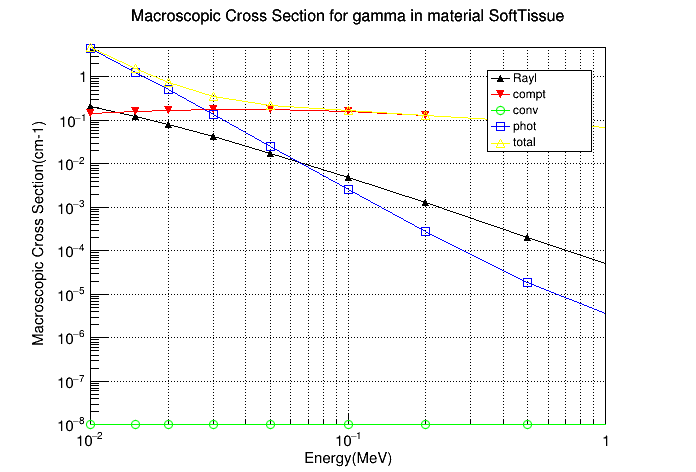
\includegraphics[width=11cm,height=7cm]{ResGra/Macroscopic_Cross_Section_for_gamma_in_material_SoftTissue.pdf}
    \centering
	\caption{Macroscopic cross-section for gamma interaction process with material SoftTissue of density 986.9 mg/cm$^3$ that fills the Liver, Kidney and Adrenal regions} 
	\label{CrossSectioPerVolumeInMaterialSoftTissueGraph}
\end{figure}

Note that the photo-electric effect is one of the processes that stop the photon by depositing all its energy probably in source region material. Whereas the Rayleigh and Compton effects give the photon more possibilities to travel then deposit more energy out of source region material, which affects the SAFs for self-absorption and cross-irradiation.

Figure \ref{fig:Resulted_Gamma_self_absorption} shows SAF values calculated for photons energy range from 0.015 to 1 MeV in self-absorption mode, where the target and source organs are the same. The SAF values for self-absorption decrease with increasing photon energy. This behavior is a result of photo-electric cross-section decreasing when the energy increases, inducing of course more chances to photons to escape from the source organ. For energies above 0.1MeV, the self-absorption SAF remains almost constant versus energy. In fact, in this energy range the photon cross-section is slightly invariable which induces the invariability of self-absorption SAFs. The difference noticed between the three organs reflects mass or density effect.

\begin{figure} [H]
\begin{subfigure}[t]{.5\textwidth}
  \centering
  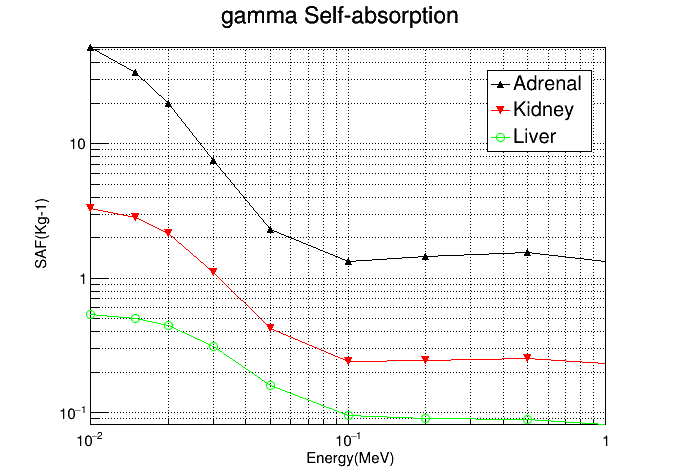
\includegraphics[width=8cm,height=5cm]{ResGra/Self_Result_SAF_gamma.pdf}
	\caption{Self-absorption SAFs in the scored regions simulated as sources.}
	\label{fig:Resulted_Gamma_self_absorption}
\end{subfigure} \hspace{.01\textwidth}
\begin{subfigure}[t]{.5\textwidth}
  \centering
  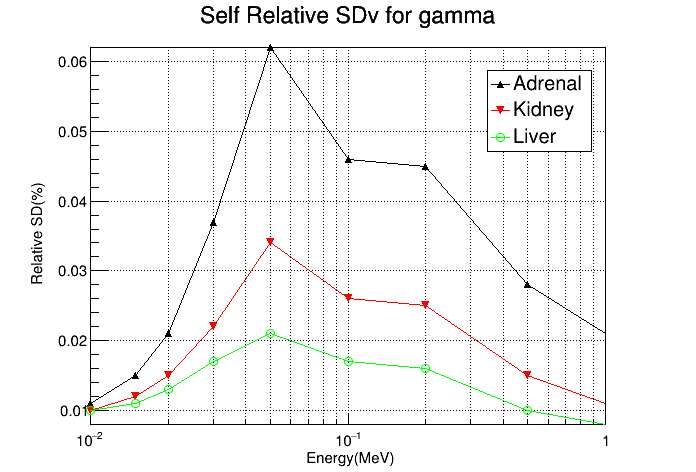
\includegraphics[width=8cm,height=5cm]{ResGra/RelativeSDv_SelfSAF.pdf}
	\caption{Relative standard deviation for self-absorption in the investigated source organs.}
	\label{fig:Self_Rel_Sdev}
	\end{subfigure}\vspace{.06\textwidth}

%\newline
\begin{subfigure}[t]{\textwidth}
  \centering
  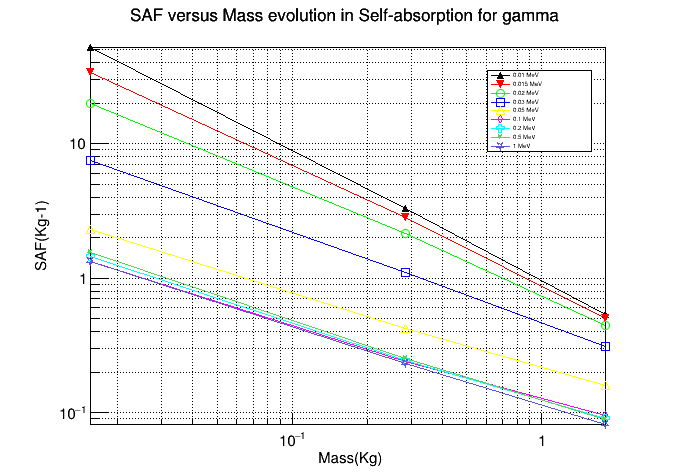
\includegraphics[width=14cm,height=9cm]{ResGra/Mass_SAFForAllEnergies_inSelfAbsorption.pdf}
	\caption{Self-absorption SAFs versus source organs mass, for Adrenal, Kidney and Liver.}
	\label{fig:SAF_versu_mass}
\end{subfigure}
%\caption{}
%\label{fig:ResultRef_Self_Irradiation}
	\caption{Self-absorption SAFs for different organs and different energies of photons. }
\end{figure}

The SAFs calculated random error values given in figure \ref{fig:Self_Rel_Sdev}, reveal that the scored self-absorption SAFs are statistically trustworthy and reliable. The achieved maximum relative SDs over the investigated energy range is roughly 0.06\% for an energy range from 0.02 to 0.1 MeV. In other words, the population(number of energy deposition times) scoring the SAFs decreases at this energy range. This can be clearly explained by the macroscopic cross-section of Compton and Rayleigh and photo-electric effects. As it shown in \ref{CrossSectioPerVolumeInMaterialSoftTissueGraph}, the compton macroscopic cross-section of SoftTissue mixture \ref{MIRDMatComp} that fills Liver, Kidney, and Adrenal volumes reaches the maximum values at the energy range from 0.02 to 0.1 MeV, giving the photon a high possibility to escape and deposit the energy out of the source organ, which leads to the increasing in SDs for self-absorption SAF. Conversely, the macroscopic cross-section of photo-electric effect continues decreasing from low to high energies.

% SD difference between organs 
The higher values of random errors are obtained for Adrenal followed by Kidney and the smallest ones are obtained for Liver. As these organs have the same density, as shown in table \ref{RegionImpleData}, the observed behavior of SDs is a consequence of variation in their volumes which are directly related to the number of contributing events in the total deposited energy. \\

On the figure \ref{fig:SAF_versu_mass} we show the influence of the organ mass on the photon SAFs for self-absorption. Hence, it can be concluded that for organs with the same density larger values of SAFs are attributed to smaller masses for all the energies in the range 0.015 - 1 MeV. 

\begin{table}[H]
\centering
\caption{Developped regions mass compared to the regions mass used in reference.}
\begin{tabular}{llll}
\hline
\textbf{Region Name} & \textbf{Mass Ref (Kg)} & \textbf{Mass(Kg)} & \textbf{Relative Diff \%} \\ \hline
Head                 & 5.08                   & 5.00              & 1.58                   \\ \hline
Skull                & 1.26                   & 1.15              & 9.39                   \\ \hline
Thyroid              & 0.02                   & 0.02              & 2.73                   \\ \hline
UpperSpine           & 0.20                   & 0.20              & 0.00                   \\ \hline
Brain                & 1.45                   & 1.45              & 0.03                   \\ \hline
Legs                 & 21.90                  & 21.72             & 0.83                   \\ \hline
LegBone              & 4.16                   & 4.15              & 0.25                   \\ \hline
Rib                  & 1.03                   & 1.03              & 0.17                   \\ \hline
Skin                 & 2.83                   & 2.78              & 2.08                   \\ \hline
Teste                & 0.04                   & 0.04              & 0.12                   \\ \hline
Trunk                & 42.70                  & 42.01             & 1.63                   \\ \hline
MiddleLowerSpine     & 0.85                   & 0.85              & 0.03                   \\ \hline
Clavicle             & 0.08                   & 0.08              & 0.27                   \\ \hline
Lung                 & 1.00                   & 1.00              & 0.05                   \\ \hline
Heart                & 0.60                   & 0.60              & 0.36                   \\ \hline
ArmBone              & 1.42                   & 1.42              & 0.11                   \\ \hline
Stomach              & 0.40                   & 0.40              & 0.17                   \\ \hline
UpperLargeIntestine  & 0.22                   & 0.24              & 7.80                   \\ \hline
LowerLargeIntestine  & 0.25                   & 0.26              & 5.91                   \\ \hline
SmallIntestine       & 1.04                   & 1.01              & 3.31                   \\ \hline
UrinaryBladder       & 0.25                   & 0.24              & 0.09                   \\ \hline
Pelvis               & 0.90                   & 0.84              & 7.59                   \\ \hline
Pancreas             & 0.06                   & 0.06              & 0.27                   \\ \hline
Liver                & 1.81                   & 1.80              & 0.31                   \\ \hline
Kidney               & 0.28                   & 0.28              & 0.05                   \\ \hline
Adrenal              & 0.02                   & 0.02              & 0.04                   \\ \hline
Spleen               & 0.17                   & 0.17              & 0.10                   \\ \hline
Thymus               & 0.02                   & 0.02              & 0.01                   \\ \hline
Uterus               & 0.07                   & 0.07              & 7.20                   \\ \hline
Ovary                & 0.01                   & 0.01              & 0.30                   \\ \hline
\end{tabular}
\label{RegionMassRefComp}
\end{table}

It can be deduced that organs with similar material compositions and mass would have very similar self-absorption SAFs values. However, the eventual differences in calculated values should be related just to the statistical errors.

\begin{figure} [H]
\begin{subfigure}[t]{.5\textwidth}
  \centering
  % include first image 
  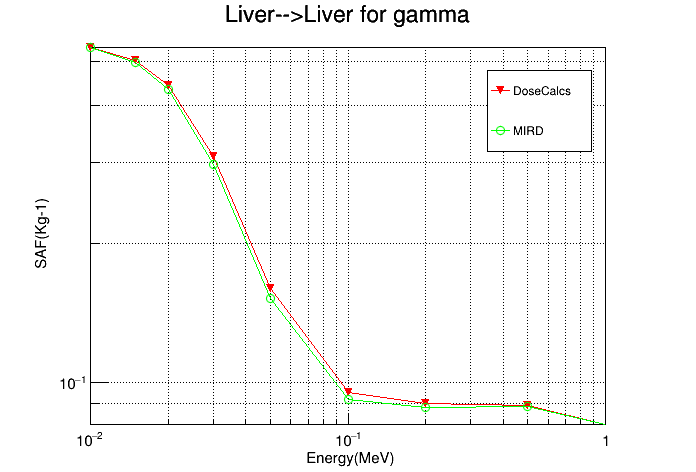
\includegraphics[width=8cm,height=5cm]{ResGra/Self_ReferenceResult_SAF_gamma_Liver_DoseCalcs_vs_MIRD.pdf}  
  \caption{Self-absorption SAFs in Liver.}
  \label{fig:SelfCompLiver}
\end{subfigure}\hspace{.01\textwidth}
\begin{subfigure}[t]{.5\textwidth}
  \centering
  % include second image
  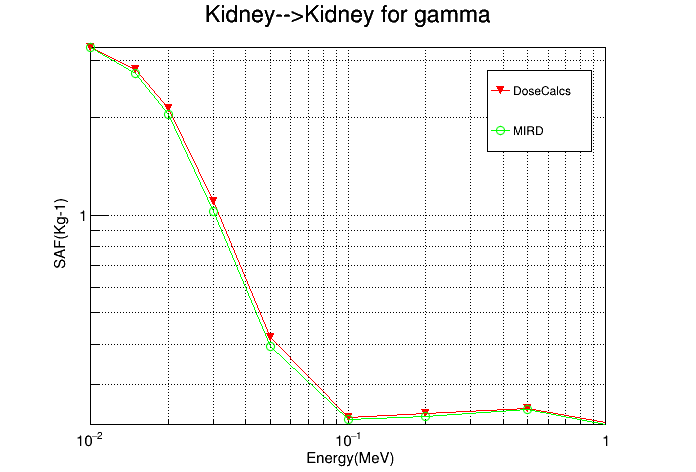
\includegraphics[width=8cm,height=5cm]{ResGra/Self_ReferenceResult_SAF_gamma_Kidney_DoseCalcs_vs_MIRD.pdf}  
  \caption{Self-absorption SAFs in Kidney.}
  \label{fig:SelfCompKidney}
\end{subfigure}\vspace{.06\textwidth}
%\newline
\begin{subfigure}[t]{.5\textwidth}
  \centering
  % include third image
  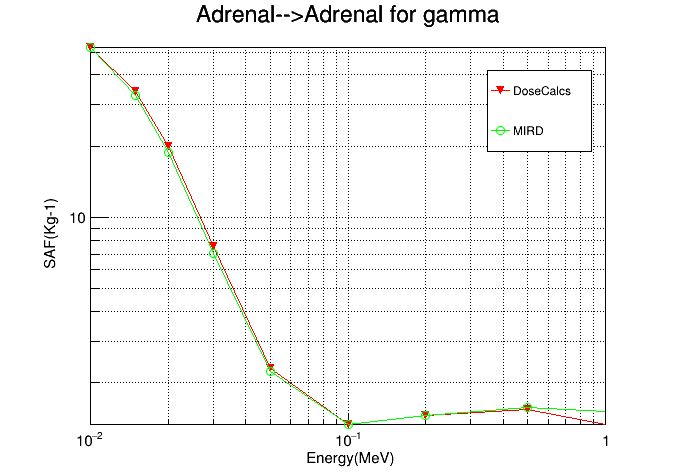
\includegraphics[width=8cm,height=5cm]{ResGra/Self_ReferenceResult_SAF_gamma_Adrenal_DoseCalcs_vs_MIRD.pdf}  
  \caption{Self-absorption SAFs in Adrenal.}
  \label{fig:SelfCompAdrenal}
\end{subfigure}\hspace{.01\textwidth}
\begin{subfigure}[t]{.5\textwidth}
  \centering
  % include fourth image
    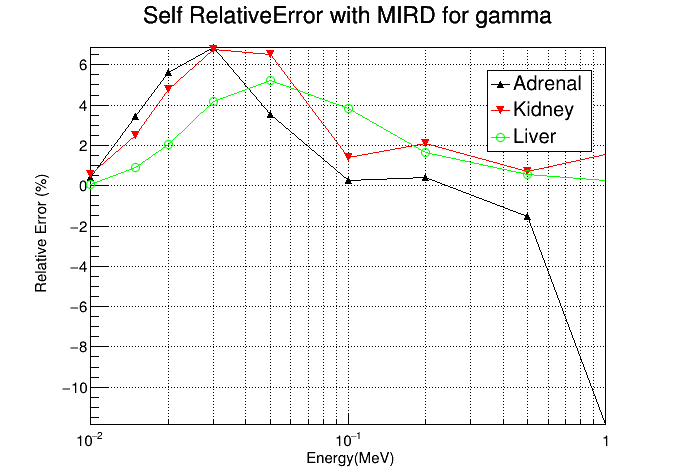
\includegraphics[width=8cm,height=5cm]{ResGra/RelativeError_Self_SAF_DoseCalcs_vs_MIRD.pdf}  
  \caption{The relative error between the DoseCalcs results and MIRD reference data.}
  \label{fig:Self_Rel_Error}
\end{subfigure}
%\caption{
%Gamma Self Absorption from in scored regions compared to MIRD data

\caption{Self-absorption SAFs comaparison between DosCalcs calculations and MIRD reference values. }
\end{figure}

The calculated self-absorption values in Liver, Kidney and Adrenal organs are presented in figures \ref{fig:SelfCompLiver}, \ref{fig:SelfCompKidney} and \ref{fig:SelfCompAdrenal} respectively and compared to reference MIRD values. It is remarked that DoseCalcs code allows to reproduce perfectly the reference data trend for the three investigated organs. Values of SAFs are also well reproduced. The observed discrepancies represented figure \ref{fig:Self_Rel_Error} are due to differences in organs masses and volumes in DoseCalcs simulated phantom and MIRD phantom; the organ shape does not have any significant effect on the self-absorption SAF estimation. In the low energy range 0.015-0.1 MeV, the SAF values calculated by DoseCalcs code overestimate slightly the reference data. This is originated from the difference in mass values \ref{RegionMassRefComp}, where in the developed GDML organs, parameters such as mass and volume can be slightly different from MIRD reference phantom data. The good agreement between self-absorption SAFs calculated values and MIRD reference data is revealed by the relative error that does not exceed 6\% for all energy range, except for Adrenal at photon energy of 1MeV, where DoseCalcs underestimates MIRD data by 12\%.

\subsubsection{Results for cross-irradiation}

The cross-irradiation SAFs in targets depends directly on the cross-sections of Compton and Rayleigh effects, and inversely on the source-target distance and cross-section of photo-electric effect. The photon traveling from the source to the target is due to Compton or Rayleigh effects. As a consequence, the cross-irradiation SAFs in various targets will decrease while photon energy decreases, due to the photo-electric cross-section which increases for low energies \ref{CrossSectioPerVolumeInMaterialSoftTissueGraph}.

\begin{figure} [H]
%\raggedright
\begin{subfigure}[t]{.5\textwidth}
  \centering
  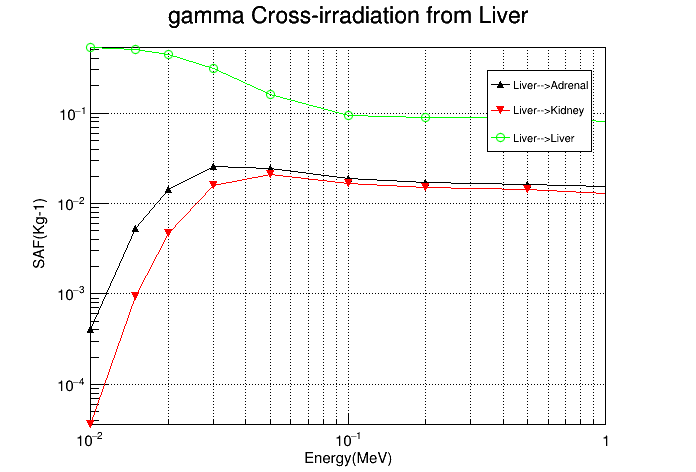
\includegraphics[width=8cm,height=5cm]{ResGra/Cross_Result_SAF_Liver_gamma.pdf}%
	\caption{Cross-irradiation SAFs from Liver source.}%
	\label{fig:CrossResultsLiver}%
\end{subfigure}\hspace{.03\textwidth}
\begin{subfigure}[t]{.5\textwidth}
  \centering
  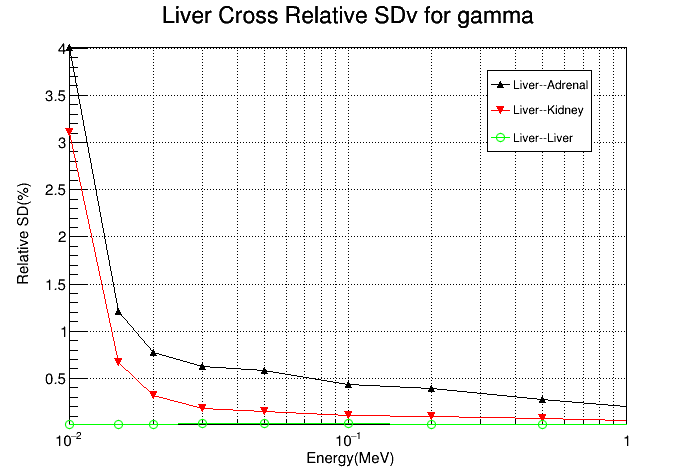
\includegraphics[width=8cm,height=5cm]{ResGra/RelativeSDv_CrossSAF_Liver.pdf}%
	\caption{Relative standard deviation(\%) for cross-irradiation from Liver.}%
	\label{fig:CrossRelSDLiver}%
	\end{subfigure}\vspace{.06\textwidth}
%\newline
\begin{subfigure}[t]{0.5\textwidth}
  \centering
  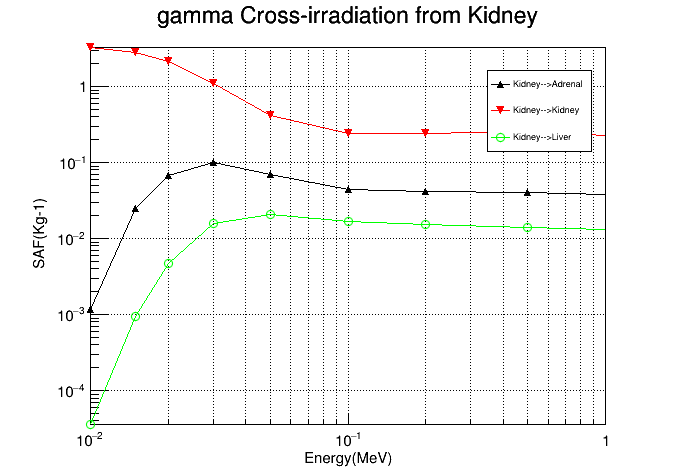
\includegraphics[width=8cm,height=5cm]{ResGra/Cross_Result_SAF_Kidney_gamma.pdf}
	\caption{Cross-irradiation SAFs from Kidney source.}
	\label{fig:CrossResultsKidney}
\end{subfigure}\hspace{.03\textwidth}
\begin{subfigure}[t]{0.5\textwidth}
  \centering
  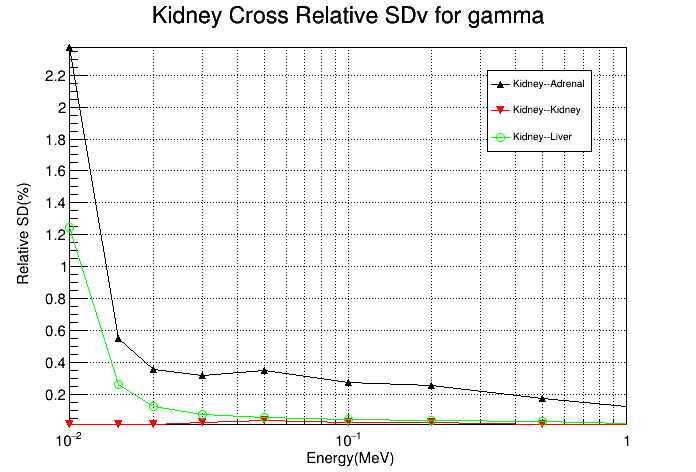
\includegraphics[width=8cm,height=5cm]{ResGra/RelativeSDv_CrossSAF_Kidney.pdf}
	\caption{Relative standard deviation(\%) for cross-irradiation from Kidney.}
	\label{fig:CrossRelSDKidney}
\end{subfigure}\vspace{.06\textwidth}
\begin{subfigure}[t]{0.5\textwidth}
  \centering
  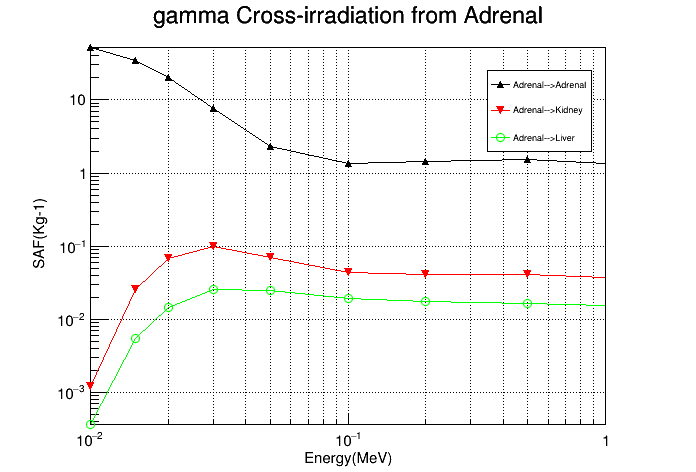
\includegraphics[width=8cm,height=5cm]{ResGra/Cross_Result_SAF_Adrenal_gamma.pdf}
	\caption{Cross-irradiation SAFs from Adrenal source.}
	\label{fig:CrossResultsAdrenal}
\end{subfigure}\hspace{.03\textwidth}
\begin{subfigure}[t]{0.5\textwidth}
  \centering
  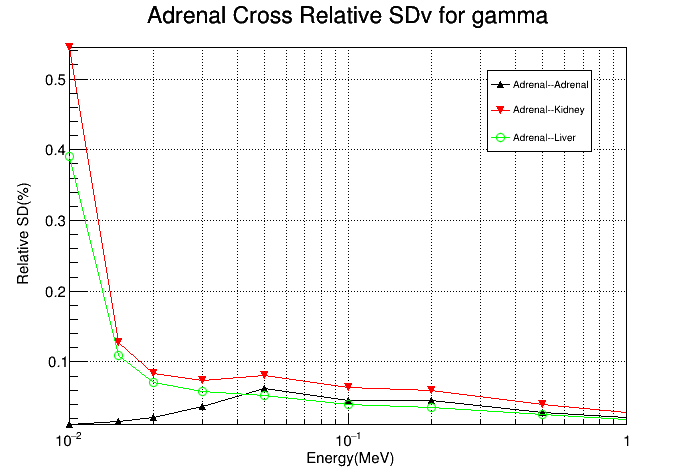
\includegraphics[width=8cm,height=5cm]{ResGra/RelativeSDv_CrossSAF_Adrenal.pdf}
	\caption{Relative standard deviation(\%) for cross-irradiation from Adrenal.}
	\label{fig:CrossRelSDAdrenal}
\end{subfigure}
\caption{DoseCalcs results for cross-irradiation SAFs and the related relative standard deviation (\%).}
%\label{fig:ResultRef_Self_Irradiation}
\end{figure}

\begin{figure} [H]
%\raggedright
\begin{subfigure}[t]{0.5\textwidth}
  \centering
  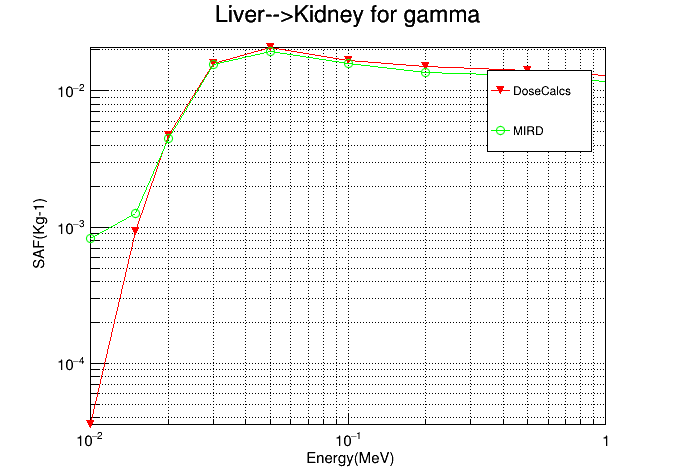
\includegraphics[width=8cm,height=5cm]{ResGra/Cross_ReferenceResult_SAF_gamma_Liver_Kidney_DoseCalcs_vs_MIRD.pdf}
	\caption{Cross-irradiation SAFs from Liver to Kidney.}
	\label{fig:CrossCompLiverKidney}
\end{subfigure}\hspace{.03\textwidth}
\begin{subfigure}[t]{0.5\textwidth}
  \centering
  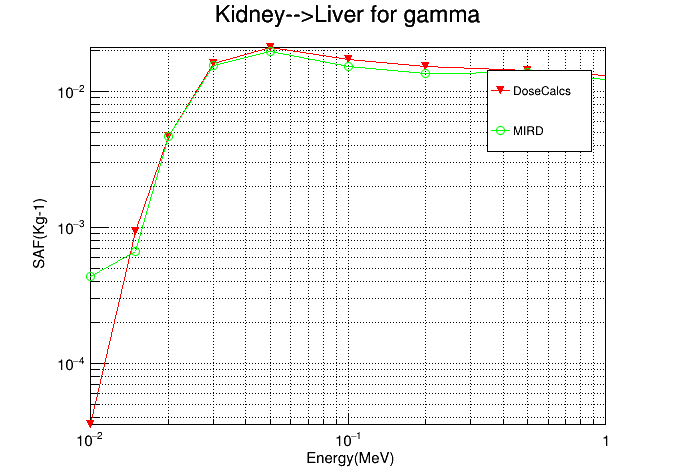
\includegraphics[width=8cm,height=5cm]{ResGra/Cross_ReferenceResult_SAF_gamma_Kidney_Liver_DoseCalcs_vs_MIRD.pdf}
	\caption{Cross-irradiation SAFs from Kidney to Liver.}
	\label{fig:CrossCompKidneyLiver}
\end{subfigure}\vspace{.06\textwidth}
\begin{subfigure}[t]{0.5\textwidth}
  \centering
  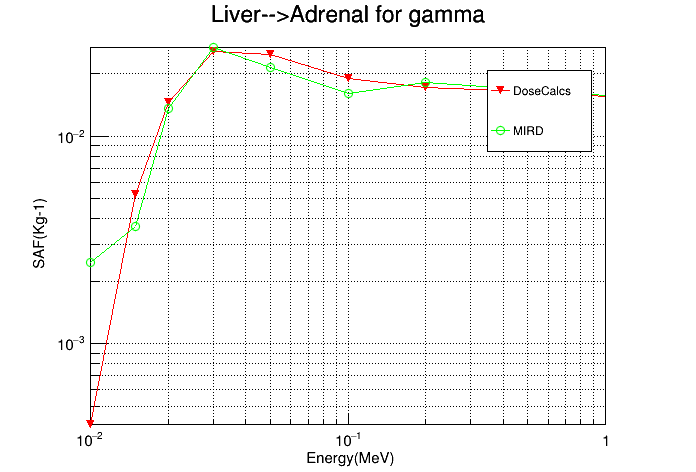
\includegraphics[width=8cm,height=5cm]{ResGra/Cross_ReferenceResult_SAF_gamma_Liver_Adrenal_DoseCalcs_vs_MIRD.pdf}
	\caption{Cross-irradiation SAFs from Liver to Adrenal.}
	\label{fig:CrossCompLiverAdrenal}
\end{subfigure}\hspace{.03\textwidth}
\begin{subfigure}[t]{0.5\textwidth}
  \centering
  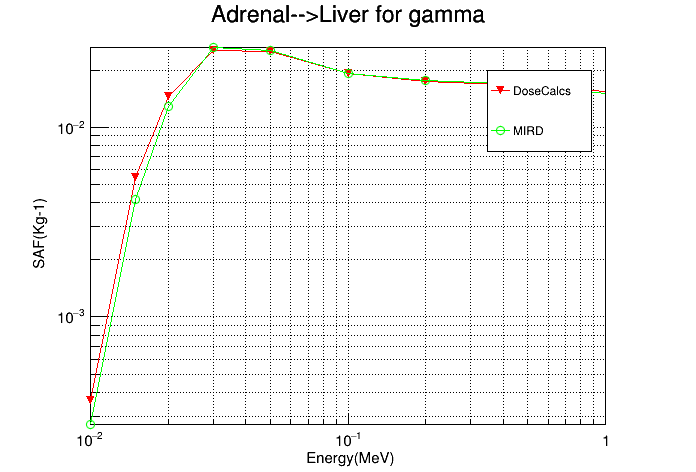
\includegraphics[width=8cm,height=5cm]{ResGra/Cross_ReferenceResult_SAF_gamma_Adrenal_Liver_DoseCalcs_vs_MIRD.pdf}
	\caption{Cross-irradiation SAFs from Adrenal to Liver.}
	\label{fig:CrossCompAdrenalLiver}
\end{subfigure}
\caption{DoseCalcs SAFs for cross-irradiation compared to the reference data to and from Liver.}
\label{fig:CrossComp}
\end{figure}

\begin{figure} [H]
%\raggedright
\begin{subfigure}[t]{0.5\textwidth}
  \centering
  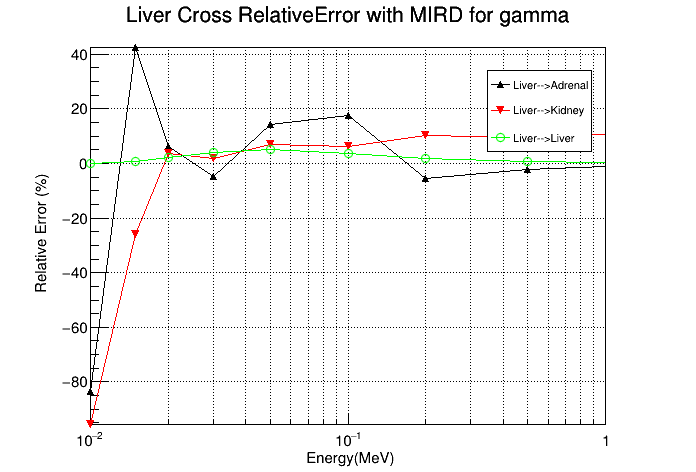
\includegraphics[width=8cm,height=5cm]{ResGra/RelativeError_Cross_SAF_Liver_DoseCalcs_vs_MIRD.pdf}
	\caption{Relative error for cross-irradiation from Liver as a source.}
	\label{fig:CrossCompErrLiver}
\end{subfigure}\hspace{.03\textwidth}
\begin{subfigure}[t]{0.5\textwidth}
  \centering
  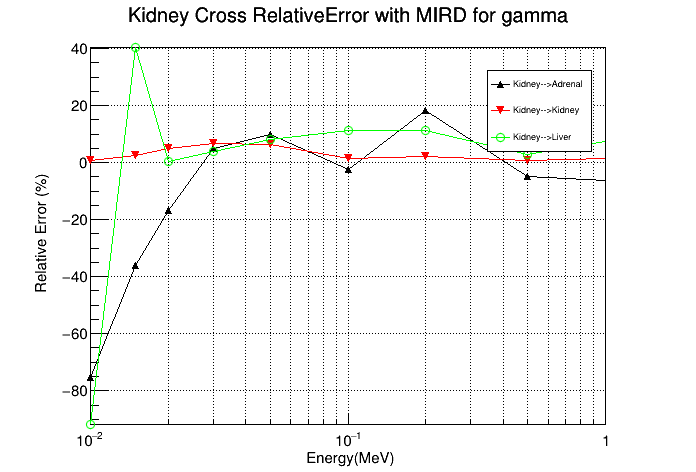
\includegraphics[width=8cm,height=5cm]{ResGra/RelativeError_Cross_SAF_Kidney_DoseCalcs_vs_MIRD.pdf}
	\caption{Relative error for cross-irradiation from Kidney as a source.}
	\label{fig:CrossCompErrKidney}
\end{subfigure}\vspace{.06\textwidth}
\begin{subfigure}[t]{\textwidth}  
\centering
  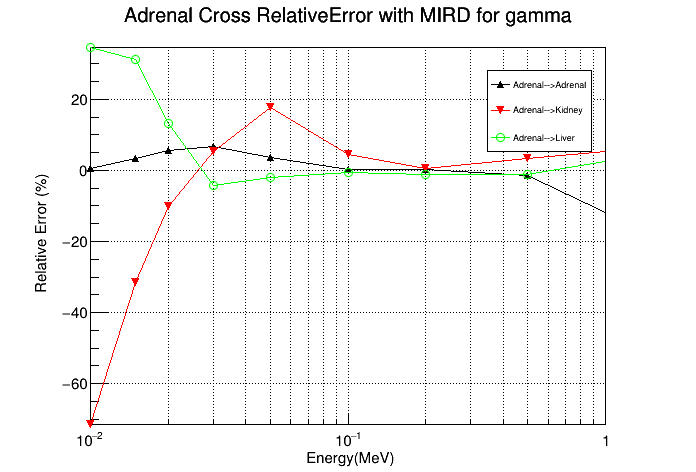
\includegraphics[width=8cm,height=5cm]{ResGra/RelativeError_Cross_SAF_Adrenal_DoseCalcs_vs_MIRD.pdf}
	\caption{Relative error for cross-irradiation from Adrenal as a source.}
	\label{fig:CrossCompErrAdrenal}
\end{subfigure}
\caption{Relative error (\%) related to the calculated cross-irradiation SAFs data from source organs such as Liver, Kidney and Adrenal.}
\label{fig:CrossCompErr}
\end{figure}

%cross SAFs values results for each source and for all targets with monte carlo error SDv:
The Specific absorbed fractions (SAFs) for photon cross-irradiation when Liver, Kidney and Adrenal as sources were displayed in figures \ref{fig:CrossResultsLiver}, \ref{fig:CrossResultsKidney} and \ref{fig:CrossResultsAdrenal}. For Liver source, at low energies, it's shown clearly that the SAFs of adrenal which has the small mass have the larger value. Likewise for high energies, the cross SAFs for adrenal and kidney stay mostly invariable.

%cross energy penetration :
For low gamma energies, the mean absorbed energy in the source organ is high, conversely, only a small quantity of the total deposit energy is absorbed in a target, because of the low energy which make the photon can't penetrate other target organs and the high value of macroscopic cross-section of photo-electric at low energies, this make absorption of photons predominates at low energies. This is indicated by the statistics in \ref{fig:CrossCompErr}, show that the estimate is unreliable and can be compensated partially by using reduction variance techniques. Additionally, the photon with low energy, can reach quickly the implicated cuts in range or energy, which make the deposit of energy locally in the source region, this explains the small values of cross-irradiation SAFs calculated by DoseCalcs compared to MIRD reference data at low energies in the figures \ref{fig:CrossCompLiverKidney}, \ref{fig:CrossCompKidneyLiver}, \ref{fig:CrossCompLiverAdrenal} and \ref{fig:CrossCompAdrenalLiver}.

Moreover, the figures in \ref{fig:CrossCompErr}, show a high relative error between DoseCalcs and reference data, this difference in cross SAFs at low energies is originated from statistical uncertainty, this random error as presented in the figures \ref{fig:CrossRelSDLiver}, \ref{fig:CrossRelSDKidney} and \ref{fig:CrossRelSDAdrenal} reveal the relative standard deviation for 0.01-0.02 MeV, where it reaches 5\%. Therefore, the insufficient agreement between the two data due also to the insufficient SAFs statistics in the scored target regions at low energies, and cannot be related to the DoseCalcs code.

%good agreement for high energies by discussing SAFs comparison for each source and by the relative error  
Otherwise, the figures in \ref{fig:CrossComp} show that calculated cross-irradiation SAFs by DoseCalcs at high energies converge to the MIRD reference data, which gives a good agreement between the two data. The relative error shown in figures \ref{fig:CrossCompErr} at energies above 0.02 MeV, is originated from the dissimilarity in shape forms of the opposite sides of source organ and target organ between the developed phantom organs in this paper and the reference.

%no agreement for low energies by discussing SAFs comparison for each source and by the relative error

\section{Conclusion}

The main objective of this study is to provide a new Geant4 based platform to perform Monte Carlo simulation and analysis of internal dosimetry problems.
DoseCalcs code has been developed to allow an easy estimation of internal dosimetry quantities using multiple geometry format, GDML, TEXT and STL, in simple steps, with powerful and facilitated utilities, yielding to study the personalized dosimetry. DoseCalcs uses segmented STL patient organs and transforms the geometry to GDML format. The user-friendly application can be run in sequential, multi-threading or MPI computation modes. Overall, the results generated by DoseCalcs for Specific Absorbed Fraction in both self-absorption and cross-irradiation with photons in Liver, Adrenal and Kidney organs are hopefuls when compared to MIRD reference data. This proves the capability of our developed DoseCalcs code in internal dosimetry, data analysis and comparison. As a perspective of this study we plan to extend the study to other organs and develop a facilitating way to estimate the most important parameters related to the patient radiation safety during nuclear medicine imaging technique.

\begin{thebibliography}{99}

%\bibitem{VFDS} IAEA, Radiation Oncology Physics: A Handbook for Teachers and Students, International Atomic Energy Agency, 2005.

%PET/CT technic:

\bibitem{AAAA} Czernin J, Schelbert H. PET/CT Imaging: Facts, opinions, hopes, and questions. J Nucl Med. 2004;45(Suppl):1S–3S.

\bibitem{BBBB} Huang B, Law MW, Khong PL. Whole-body PET/CT scanning: estimation of radiation dose and cancer risk. Radiology 2009; 251 : 166-74.

\bibitem{ICRP103} ICRP. The 2007 Recommendations of the International Commission on Radiological Protection, ICRP Publication 103. Ann ICRP. 2007;37:1–332.


%Geant4:

\bibitem{Geant4} S. Agostinelli, J. Allison, K. Amako, J. Apostolakis, H. Araujo, P. Arce, et al., “Geant4 - a simulation toolkit”, NIM A, vol. 506, no. 3, pp. 250-303, 2004.

%\bibitem{FFFF} J. Allison, K. Amako, J. Apostolakis, H. Araujo, P. Arce Dubois, M. Asai, et al., “Geant4 developments and applications”, IEEE Trans. Nucl. Sci., vol. 53, no. 1, pp. 270-278, Feb. 2006.

%\bibitem{PhysicsList} “Guide For Physics Lists,” n.d., 65.

\bibitem{PhysicsRefGuide} Geant4 Physics Reference Manual, 2008, Geant4 Group.

%GDML TEXT STL :

\bibitem{GDMLFormat} R Chytracek, J. Mccormick, W. Pokorski, and G. Santin, “Geometry Description Markup Language for Physics Simulation and Analysis Applications”, IEEE Trans. Nucl. Sci., vol. 53, no. 5, pp. 2892-2896, Oct. 2006.

\bibitem{TEXTFormat} TEXT file geometry manual, Credit/Citations for Data Files Distributed With Geant4, 2009, Geant4 Group.

\bibitem{STLFormat} I. Stroud, P.C. Xirouchakis, STL and extensions, Advances in Engineering Software, Volume 31, Issue 2, 2000, Pages 83-95, ISSN 0965-9978, https://doi.org/10.1016/S0965-9978(99)00046-0. (http://www.sciencedirect.com/science/article/pii/S0965997899000460)

\bibitem{OLINDAEXE} M.G. Stabin, R.B. Sparks, E. Crowe OLINDA/EXM: the second-generation computer software for internal dose assessment in nuclear medicine J Nucl Med, 46 (2005), pp. 1023-1027

\bibitem{Gate} S. Jan, G. Santin, D. Strul, S. Staeklens, K. Assie, D. Autret, et al. GATE: A simulation toolkit for PET and SPECT
Phys Med Biol, 49 (2004), pp. 4543-4561

\bibitem{MCNPCode} F.B. Brown MCNP - a general Monte Carlo N-particle transport code v. R. LA-UR-03-1987 Los Alamos National Laboratory, Los Alamos NM (2003)

\bibitem{NISTDataBase} National Institute of Standards \& Technology Standard Reference Material 2461 – Standard Cartridge Case NIST, Gaithersburg, MD (2012)

%MPI G4MPI and MT

\bibitem{MPI} M. Snir and W. Gropp, MPI the complete reference, Cambridge:MIT Press, 1998.

\bibitem{G4MPI} Dotti, Andrea, Makoto Asai, Guy Barrand, Ivana Hrivnacova, and Koichi Murakami. “Extending Geant4 Parallelism with External Libraries (MPI, TBB) and Its Use on HPC Resources.” ArXiv:1605.01792 [Hep-Ex, Physics:Physics], May 5, 2016. http://arxiv.org/abs/1605.01792.

\bibitem{MT} Ahn, S., Apostolakis, J., Cosmo, G., Nowak, A., Asai, M., Brandt, D., Dotti, A., Coopermann, G., Dong, X., \& Jun, Soon Yung (2013). Geant4-MT: bringing multi-threading into Geant4 production. France: EDP Sciences.

% SUV 
\bibitem{SUV} Thie JA. Understanding the standardized uptake value, its methods, and implications for usage. J Nucl Med. 2004 Sep;45(9):1431-4. PMID: 15347707.

%Root

\bibitem{ROOT} Rene Brun and Fons Rademakers, ROOT - An Object Oriented Data Analysis Framework, Proceedings AIHENP'96 Workshop, Lausanne, Sep. 1996, Nucl. Inst. \& Meth. in Phys. Res. A 389 (1997) 81-86.

%phantoms Reference Data
\bibitem{MIRDRefPhantomData} Snyder WS, Fisher HL, Ford MR, Warner GG (1969) Estimates of absorbed fractions for monoenergetic photon sources uniformly distributed in various organs of a heterogeneous phantom. J Nucl Med 3(Suppl):7–52

\bibitem{MIRDRefSAFData} W. S. Snyder, M. R. Ford M R, G. G. Wamer and H. L. Fisher, “MIRD Pamphlet No. 5 Revised, Estimates of absorbed fractions for monoenergetic photon sources uniformly distributed in various organs of a heterogeneous phantom”, J. Nucl. Med. Suppl., no. 3, pp. 5-52, 1969.

\bibitem{G4HumanPhantom} Guatelli, S., Mascialino, B., Pia, M. Grazia. \& Pokorski, W. (2006). Geant4 antropomorphic phantoms. In B. Phlips (Eds.), IEEE Nuclear Science Symposium Conference Record (pp. 1359-1362). New Jersey, United States: IEEE.

%\bibitem{PPPP} M. Cristy and K. F. Eckerman, Specific absorbed fractions of energy at various ages from internal photon sources, ORNL/TM-8381/V1, Apr. 1987.

%Monte carlo 

\bibitem{ExplorMonteCarlo} Dunn, William L., and J. Kenneth Shultis. Exploring Monte Carlo Methods. Amsterdam ; Boston: Elsevier/Academic Press, 2012.

%ICRP Methods 
\bibitem{ICRPMethod} ICRP, 201Y. The ICRP Computational Framework for Internal Dose Assessment for Reference Workers: Specific Absorbed Fractions. ICRP Publication 1XX, Ann. ICRP 4X (0).


\end{thebibliography}

\end{document}
